\documentclass{article}
%----------------------------------------------------------------------
\usepackage[polish]{babel}
\usepackage[utf8]{inputenc}
\usepackage[T1]{fontenc}
\usepackage[a4paper,top=2cm,bottom=2cm,left=3cm,right=3cm,marginparwidth=1.75cm]{geometry}
\usepackage{amsmath}
\usepackage{amsthm}
\usepackage{amssymb}
\usepackage{graphicx}
\usepackage[colorlinks=true, allcolors=black]{hyperref}
\usepackage{blindtext}
\usepackage{nomencl}
\usepackage{amsfonts}
\usepackage{listings}
\usepackage{xcolor}
\usepackage{float}
\usepackage{etoolbox}
\usepackage{tabularx}
\usepackage{tabularray}
\usepackage{array}
\usepackage{enumitem}
\usepackage{subcaption}
\usepackage{tikz}
\usetikzlibrary{graphs, graphs.standard,decorations.pathreplacing, positioning, calc}
%----------------------------------------------------------------------
\usepackage{algorithm}
\usepackage{algpseudocode}

\usepackage{csquotes}
\usepackage[backend=biber, style=numeric]{biblatex}
\addbibresource{refs.bib}

% ----------------------------------------------------
\theoremstyle{definition}
\newtheorem{definition}{Definicja}[section]
\newtheorem{example}[definition]{Przykład}

\theoremstyle{plain}
\newtheorem{properties}[definition]{Własności}
\newtheorem{theorem}[definition]{Twierdzenie}
\newtheorem{conclusion}[definition]{Wniosek}
\newtheorem{lemma}[definition]{Lemat}

\theoremstyle{remark}
\newtheorem*{remark}{Uwaga}
% ----------------------------------------------------

\begin{document}

\begin{titlepage}
    \centering
    \vspace{1.5cm}
    
\includegraphics[width=0.9\textwidth]{university-logo.png} \\
    \vspace{1cm}
    {\fontsize{30}{20}\selectfont \textbf{Algorytmy zaawansowane} \par}
    \vspace{1.5cm}
    {\fontsize{25}{20}\selectfont \textbf{Komiwojażer}\par}
    \vspace{1cm}
    {\fontsize{20}{20}\selectfont Porównanie dwóch algorytmów aproksymacyjnych znajdujących rozwiązanie problemu Komiwojażera \par}
    \vspace{2cm}
    {\fontsize{18}{20}\selectfont Raport końcowy\par}
    \vspace{1cm}
    {\fontsize{12}{20}\selectfont Zespół: \\ inż. Marcin Cieszyński \\ inż. Radosław Głasek \\ inż. Adam Grącikowski \par}
    \vspace{1cm}
    {\fontsize{12}{20}\selectfont Prowadzący: \\ dr Michał Tuczyński \par}
    
    \vfill
    Oświadczamy, że niniejsza praca, stanowiąca podstawę do uznania osiągnięcia efektów uczenia się z przedmiotu \textit{Algorytmy zaawansowane}, została wykonana samodzielnie. 

    \vspace{1cm}
    
    Warszawa, \today
    
\end{titlepage}

%----------------------------------------------------------------------
\tableofcontents
\newpage

%----------------------------------------------------------------------
\section{Wstęp}

Problem komiwojażera (ang. \textit{Traveling Salesperson Problem}, TSP) to jeden z klasycznych problemów optymalizacji kombinatorycznej, należący do klasy problemów NP-trudnych.

\subsection{Cel projektu}

Przedmiotem projektu jest implementacja oraz szczegółowe porównanie dwóch algorytmów aproksymacyjnych rozwiązujących metryczną wersję problemu komiwojażera. Porównanie ma na celu ewaluację obu podejść pod kątem jakości zwracanych rozwiązań w stosunku do czasu ich wykonania na instancjach testowych o zróżnicowanej wielkości~\cite{dokumentacja_wstepna_tsp}.

\subsection{Przedstawienie problemu}

Zadanie komiwojażera polega na znalezieniu najkrótszej możliwej trasy, która zaczyna się w wybranym punkcie, odwiedza dokładnie jeden raz każdy z pozostałych punktów, a następnie wraca do miejsca startu.

W ujęciu grafowym problem ten modeluje się za pomocą pełnego grafu nieskierowanego ważonego $G = (V, E)$, gdzie $V$ to zbiór wierzchołków reprezentujących lokalizacje, a $E$ to zbiór krawędzi łączących każdą parę wierzchołków. Każdej krawędzi przypisana jest waga za pomocą funkcji kosztu $c: E \to \mathbb{N}$. Zastosowanie dziedziny liczb naturalnych oznacza, że operujemy na całkowitoliczbowych, nieujemnych wartościach odległości. Naszym celem jest znalezienie cyklu Hamiltona $C$ o minimalnym sumarycznym koszcie krawędzi.

Wersja metryczna problemu, którą rozpatrujemy w tym projekcie, nakłada na funkcję kosztu dodatkowe ograniczenia, upodabniające graf do rzeczywistej przestrzeni fizycznej. Najważniejszym z nich jest \textbf{nierówność trójkąta}. Oznacza ona, że bezpośrednia podróż z wierzchołka $u$ do $w$ nigdy nie jest droższa niż podróż przez jakikolwiek wierzchołek pośredni $v$. Formalnie dla każdych trzech wierzchołków $u, v, w \in V$ zachodzi:

$$c(u, w) \le c(u, v) + c(v, w)$$

\noindent
Dodatkowo zakładamy symetrię, czyli $c(u, v) = c(v, u)$.

\newpage
\section{Zmiany w stosunku do dokumentacji wstępnej}
Nie wprowadzono zmian w stosunku do dokumentacji wstępnej. 

\section{Instrukcja użytkownika}

Aplikacja została zrealizowana w środowisku .NET 9 jako program konsolowy, który wczytuje instancję problemu z pliku tekstowego. Wynik działania algorytmu jest domyślnie wypisywany na standardowe wyjście (konsolę) w czytelnej dla użytkownika formie, a opcjonalnie może zostać zapisany do pliku tekstowego.

\subsection{Składnia poleceń}

Podstawowa składnia wywołania programu (zakładając, że skompilowany plik wykonywalny nosi nazwę \texttt{tsp-approximation.exe}) prezentuje się następująco:

\begin{verbatim}
tsp-approximation.exe <FilePath> [opcje]
\end{verbatim}

\subsubsection{Dostępne argumenty i flagi}

Program przyjmuje jeden argument pozycyjny oraz dodatkowe flagi modyfikujące jego zachowanie:

\begin{itemize}
    \item \textbf{\texttt{<FilePath>}} (argument wymagany) -- argument pozycyjny podawany bezpośrednio po nazwie programu. Określa ścieżkę do pliku tekstowego zawierającego macierz sąsiedztwa grafu.
    \item \textbf{\texttt{-o, ---output <ścieżka>}} (argument opcjonalny) -- pozwala na zdefiniowanie ścieżki do pliku wyjściowego, w którym zapisany zostanie wynik działania wybranego algorytmu. Jeśli parametr ten zostanie pominięty, wynik zostanie wypisany wyłącznie na standardowe wyjście (konsolę).
    \item \textbf{\texttt{-d, ---double-tree}} (flaga opcjonalna) -- jej podanie wymusza użycie algorytmu \\ 2-aproksymacyjnego. Jeśli flaga nie zostanie ustawiona, program domyślnie wykorzysta algorytm Christofidesa.
    \item \textbf{\texttt{---help}} -- wbudowana flaga, która wyświetla na ekranie krótką instrukcję obsługi i opisy dostępnych argumentów w języku angielskim.
\end{itemize}

\subsection{Przykłady użycia}

\subsubsection*{Uruchomienie domyślne (algorytm Christofidesa):}

\begin{verbatim}
tsp-approximation.exe graph.txt
\end{verbatim}

\noindent
Program wczyta graf z pliku \texttt{graph.txt}, wykona obliczenia za pomocą algorytmu Christofidesa, a wynik zaprezentuje bezpośrednio w konsoli.

\subsubsection*{Uruchomienie algorytmu podwójnego drzewa z zapisem do pliku:}
\begin{verbatim}
tsp-approximation.exe graph.txt -d -o result.txt
\end{verbatim}
Program wykorzysta algorytm 2-aproksymacyjny (\texttt{-d}) i zapisze sformatowany cykl Hamiltona oraz jego koszt do pliku \texttt{result.txt} (\texttt{-o}).

\subsubsection*{Alternatywny zapis z pełnymi nazwami flag:}
\begin{verbatim}
tsp-approximation.exe graph.txt --double-tree --output result.txt
\end{verbatim}
Wywołanie to jest w pełni równoważne z przykładem drugim, ale wykorzystuje długie aliasy poleceń.

\subsection{Format danych wejściowych}

Plik wejściowy jest standardowym plikiem tekstowym. Jego struktura opiera się na następujących zasadach:
\begin{itemize}
    \item W pierwszej linii znajduje się pojedyncza liczba całkowita dodatnia $N$, określająca całkowitą liczbę wierzchołków w grafie.
    \item W kolejnych $N$ liniach znajduje się macierz sąsiedztwa modelująca graf pełny. Każdy wiersz zawiera dokładnie $N$ wartości oddzielonych białymi znakami (pojedynczą spacją lub tabulatorem).
\end{itemize}

\noindent
Wartości w macierzy reprezentują wagi krawędzi (odległości) i są liczbami naturalnymi. Macierz jest symetryczna, posiada zera na głównej przekątnej, a zapisane w niej odległości spełniają nierówność trójkąta.

\subsection{Format danych wyjściowych}

Plik wyjściowy jest standardowym plikiem tekstowym. Jego struktura opiera się na następujących zasadach:

\begin{itemize}
    \item Pierwsza linia rozpoczyna się od frazy ,,\texttt{Total Distance:\ }'', po której następuje całkowity koszt znalezionego rozwiązania (suma wag krawędzi tworzących cykl Hamiltona).
    \item Druga linia rozpoczyna się od frazy ,,\texttt{Route:\ }'', po której następuje reprezentacja wyznaczonego cyklu Hamiltona. Identyfikatory wierzchołków wypisane są w kolejności odwiedzania i rozdzielone znakiem pauzy (\texttt{-}). Pierwszy i ostatni wierzchołek w tej linii są identyczne, domykając cykl.
\end{itemize}

\subsection{Przykłady wejścia i wyjścia}

Przeanalizujemy zawartość pliku wejściowego oraz wyjściowego na przykładzie grafu $G$ przedstawionego na Rysunku \ref{rys:przyklad}. 

\begin{figure}[H]
    \centering
    \begin{tikzpicture}[scale=1.8, auto, swap]
        \foreach \i in {0,...,4}
            \node[circle, draw, fill=gray!10] (\i) at ({90+72*\i}:1.5) {\i};

        \draw (0) -- (1) node[midway, above left] {1};
        \draw (1) -- (2) node[midway, left] {1};
        \draw (2) -- (3) node[midway, below] {1};
        \draw (3) -- (4) node[midway, right] {1};
        \draw (4) -- (0) node[midway, above right] {1};

        \draw[dashed, gray] (0) -- (2) node[pos=0.3, left, black] {2};
        \draw[dashed, gray] (0) -- (3) node[pos=0.3, right, black] {2};
        \draw[dashed, gray] (1) -- (3) node[pos=0.7, right, black] {2};
        \draw[dashed, gray] (1) -- (4) node[pos=0.5, below, black] {2};
        \draw[dashed, gray] (2) -- (4) node[pos=0.7, above, black] {2};
    \end{tikzpicture}
    \caption{Przykładowy graf wejściowy $G$.}
    \label{rys:przyklad}
\end{figure}

\noindent
Graf składa się z pięciu wierzchołków ($N=5$). Krawędzie ułożone wzdłuż obwodu pięciokąta mają wagę $1$, natomiast wszystkie ,,przekątne'' (łączące wierzchołki niebędące bezpośrednimi sąsiadami na obwodzie) mają wagę $2$. Warto zauważyć, że wszystkie wagi krawędzi to liczby naturalne i spełniona jest tu nierówność trójkąta. \\

\noindent
Zawartość pliku wejściowego dla grafu $G$ przedstawia Rysunek \ref{lst:input}.

\begin{figure}[H]
\begin{verbatim}
5
0 1 2 2 1
1 0 1 2 2
2 1 0 1 2
2 2 1 0 1
1 2 2 1 0
\end{verbatim}
\caption{Zawartość pliku wejściowego dla grafu $G$.}
\label{lst:input}
\end{figure}

Wynik działania programu dla powyższej instancji został zilustrowany na Rysunku \ref{lst:output}. Pierwsza linia pliku wyjściowego precyzuje całkowity koszt znalezionej trasy, wynoszący w tym przypadku $5$. Jest to suma wag pięciu krawędzi wchodzących w skład wyznaczonego cyklu. Druga linia określa dokładną kolejność odwiedzania wierzchołków. 

\begin{figure}[H]
\begin{verbatim}
Total Distance: 5
Route: 0-1-2-3-4-0
\end{verbatim}
\caption{Zawartość pliku wyjściowego dla grafu $G$.}
\label{lst:output}
\end{figure}

\noindent
W prezentowanym przykładzie wyznaczona ścieżka (\texttt{0-1-2-3-4-0}) przebiega wyłącznie po krawędziach o wadze $1$ (Rysunek \ref{rys:optymalny}).

\begin{figure}[H]
    \centering
    \begin{tikzpicture}[scale=1.8]
        \foreach \i in {0,...,4}
            \node[circle, draw, fill=gray!10] (\i) at ({90+72*\i}:1.5) {\i};

        \draw (0) -- (1) node[midway, above left] {1};
        \draw (1) -- (2) node[midway, left] {1};
        \draw (2) -- (3) node[midway, below] {1};
        \draw (3) -- (4) node[midway, right] {1};
        \draw (4) -- (0) node[midway, above right] {1};
        
        \draw[dashed, gray] (0) -- (2) node[pos=0.3, left, black] {2};
        \draw[dashed, gray] (0) -- (3) node[pos=0.3, right, black] {2};
        \draw[dashed, gray] (1) -- (3) node[pos=0.7, right, black] {2};
        \draw[dashed, gray] (1) -- (4) node[pos=0.5, below, black] {2};
        \draw[dashed, gray] (2) -- (4) node[pos=0.7, above, black] {2};
        
        \draw[line width=2pt, blue] (0) -- (1) -- (2) -- (3) -- (4) -- (0);
        
    \end{tikzpicture}
    \caption{Rozwiązanie zapisane w pliku wyjściowym.}
    \label{rys:optymalny}
\end{figure}

\newpage
\section{Generowanie instancji testowych}

Aplikacja została zrealizowana w środowisku .NET 9 jako program konsolowy.

\subsection{Składnia poleceń}

Podstawowa składnia wywołania programu prezentuje się następująco:

\begin{verbatim}
tsp-generator.exe --start <wartość> [opcje]
\end{verbatim}

\subsubsection{Dostępne argumenty i flagi}

Program wymaga podania rozmiaru startowego oraz przyjmuje szereg argumentów opcjonalnych modyfikujących proces generowania:

\begin{itemize}
    \item \textbf{\texttt{---start <wartość>}} (argument wymagany) -- określa początkową liczbę wierzchołków dla pierwszej instancji w generowanej serii.
    
    \item \textbf{\texttt{---step <wartość>}} (argument opcjonalny, domyślnie: 1) -- rozmiar kroku, o jaki zwiększana jest liczba wierzchołków w każdej kolejnej generowanej instancji.
    
    \item \textbf{\texttt{-c, ---count <wartość>}} (argument opcjonalny, domyślnie: 1) -- łączna liczba instancji (plików) do wygenerowania w ramach jednego uruchomienia.
    
    \item \textbf{\texttt{-s, ---size <wartość>}} (argument opcjonalny, domyślnie: 1000) -- maksymalna wartość współrzędnych (na osiach X i Y) dla losowanych wierzchołków.
    
    \item \textbf{\texttt{-d, ---dir <ścieżka>}} (argument opcjonalny, domyślnie: \texttt{data}) -- ścieżka do katalogu docelowego, w którym zostaną zapisane pliki z rozszerzeniem \texttt{.txt}.
    
    \item \textbf{\texttt{---help}} -- wyświetla na standardowym wyjściu instrukcję obsługi programu.
\end{itemize}

\subsection{Przykłady użycia}

\subsubsection*{Uruchomienie podstawowe (pojedyncza instancja)}

\begin{verbatim}
tsp-generator.exe --start 50
\end{verbatim}

\noindent
Program wygeneruje pojedynczy graf składający się z 50 wierzchołków, wylosuje współrzędne z przedziału od 0 do 1000 i zapisze wynik w domyślnym katalogu \texttt{data}.

\subsubsection*{Generowanie serii instancji testowych}

\begin{verbatim}
tsp-generator.exe --start 100 --step 10 -c 10 -d test_set
\end{verbatim}

\noindent
Polecenie wygeneruje serię 10 plików (\texttt{-c 10}), zaczynając od rozmiaru 100 wierzchołków (\texttt{--start 100}) i zwiększając go o 10 w każdym kolejnym kroku (\texttt{--step 10}). Pliki zostaną zapisane w katalogu \texttt{test\_set} (\texttt{-d}).

\subsubsection*{Generowanie na mniejszej płaszczyźnie współrzędnych}

\begin{verbatim}
tsp-generator.exe --start 20 --size 500
\end{verbatim}

\noindent
Program wygeneruje graf 20-wierzchołkowy, w którym maksymalna wartość współrzędnych punktów na osiach X i Y nie przekroczy 500 (\texttt{--size}).

\newpage
\section{Opis eksperymentów}
\label{sec:opis_testow}

W celu przeprowadzenia kompleksowej analizy oraz walidacji zaimplementowanych algorytmów aproksymacyjnych, przygotowano zestaw instancji testowych. Zbiór ten został podzielony na trzy kategorie (znajdujące się w katalogu \texttt{examples/}):

\begin{itemize}
    \item Losowe instancje o małym rozmiarze (\path{examples/random/small}).
    \item Losowe instancje o dużym rozmiarze (\path{examples/random/large}).
    \item Instancje referencyjne z biblioteki TSPLIB~\cite{reinelt1991tsplib, tsplib_mastqe} (\path{examples/tsplib}).
\end{itemize}

\subsection{Losowe instancje o małym rozmiarze}

Pierwsza grupa testowa obejmuje 41 wygenerowanych losowo instancji problemu, dla których liczba wierzchołków $n$ zawiera się w przedziale od $n=10$ do $n=50$. Pliki z danymi przyjmują konwencję nazewnictwa \texttt{gen\_n\{liczba\_wierzcholkow\}.txt} (np. \texttt{gen\_n0010.txt}). Ze względu na minimalny krok przyrostu rozmiaru instancji, wynoszący 1 wierzchołek, zbiór ten jest wykorzystywany do szczegółowej analizy zachowania algorytmów na grafach o niewielkich rozmiarach.

\subsection{Losowe instancje o dużym rozmiarze}

Druga grupa testowa składa się z 41 wygenerowanych losowo instancji, obejmujących grafy o rozmiarach od $n=100$ do $n=500$ wierzchołków. W tym przypadku krok przyrostu wynosi 10 wierzchołków. Konwencja nazewnictwa plików jest tożsama z instancjami małymi (np. \texttt{gen\_n0100.txt}). Zbiór ten ma na celu weryfikację skalowalności oraz analizę złożoności czasowej algorytmów.

\subsection{Instancje referencyjne z biblioteki TSPLIB}

Trzecią grupę testową stanowi 40 referencyjnych instancji problemu komiwojażera pochodzących biblioteki TSPLIB. Pliki w tej podgrupie wykorzystują konwencję:

\begin{center}
\texttt{n\{liczba\_wierzcholkow\}o\{dystans\_optymalny\}.txt}
\end{center}

\noindent
Taki format (np. \texttt{n51o426.txt}) pozwala na automatyczne odczytanie długości optymalnej trasy bezpośrednio z nazwy pliku.

\subsection{Metodologia pomiarów}

W ramach przyjętej metodologii badawczej, każda z wyżej opisanych instancji testowych została przetworzona przy użyciu obu analizowanych algorytmów: algorytmu 2-aproksymacyjnego (bazującego na podwójnym drzewie rozpinającym) oraz algorytmu Christofidesa. 

Architektura przeprowadzanych eksperymentów numerycznych została zaprojektowana w sposób umożliwiający ewaluację dwóch wskaźników wydajności:

\begin{itemize}
    \item \textbf{Złożoność obliczeniowa:} Czas wykonania mierzony jest przekrojowo na seriach losowych instancji (małych i dużych). Podejście to pozwala na zaobserwowanie dynamiki wzrostu czasu wykonania algorytmów w funkcji rosnącej liczby wierzchołków badanych grafów.
    \item \textbf{Jakość aproksymacji:} Weryfikowana z wykorzystaniem instancji z rodziny TSPLIB. Dzięki znajomości wartości optimum globalnego, możliwe jest precyzyjne określenie, na ile wygenerowane przez algorytmy rozwiązanie przybliżone odbiega od optymalnego.
\end{itemize}

\newpage
\section{Wyniki i wnioski}
\label{sec:wyniki_i_wnioski}

W poniższym rozdziale zaprezentowano zestawienie oraz interpretację wyników uzyskanych w trakcie testowania zaimplementowanych algorytmów. Analiza została podzielona na dwa główne aspekty: badanie złożoności obliczeniowej oraz ocenę jakości otrzymywanych rozwiązań (współczynnika aproksymacji).

\subsection{Złożoność obliczeniowa i czas wykonania}
\label{subsec:zlozonosc_czasowa}

Pomiary czasu wykonania (wyrażone w milisekundach) pozwalają na weryfikację teoretycznych złożoności obliczeniowych oraz ocenę narzutu czasowego wynikającego ze specyfiki poszczególnych operacji składowych badanych algorytmów.

\subsubsection{Analiza małych instancji losowych}
\label{subsubsec:czas_male_instancje}

Na podstawie przeprowadzonych eksperymentów dla zbioru instancji małych, można zaobserwować wyraźne różnice w charakterystyce działania obu badanych algorytmów. Wyniki pomiarów dla tej grupy zostały zagregowane na wykresie porównawczym (Rysunek \ref{fig:small_time_complexity}).

Algorytm 2-aproksymacyjny charakteryzuje się bardzo krótkim i relatywnie stabilnym czasem działania. W badanym przedziale od $n=10$ do $n=50$ wierzchołków, czas wykonania rośnie w sposób łagodny i przewidywalny, osiągając w wartościach szczytowych około $0{,}25$ milisekundy dla $n=49$. Zmienność czasu pomiędzy kolejnymi iteracjami (pojedynczymi przyrostami liczby wierzchołków) jest minimalna. Świadczy to o niskim koszcie obliczeniowym podstawowych kroków tego algorytmu -- wyznaczania minimalnego drzewa rozpinającego (MST).

Z kolei algorytm Christofidesa okazuje się zauważalnie bardziej wymagający pod względem czasu procesora, co uwidacznia się nawet w przypadku tak niewielkich grafów. O ile dla najmniejszych instancji ($n < 25$) czasy wykonania obu algorytmów pozostają zbliżone i rzadko przekraczają $0{,}3$ ms, o tyle w miarę wzrostu rozmiaru problemu, krzywa algorytmu Christofidesa ulega silnemu rozwarstwieniu względem algorytmu 2-aproksymacyjnego. Dodatkowo, heurystyka ta charakteryzuje się wysoką wariancją czasu wykonania –- na wykresie widoczne są gwałtowne skoki, na przykład dla $n=40$ (niemal $1{,}2$ ms) czy $n=47$ (blisko $1{,}9$ ms).

Zaobserwowana dysproporcja wynika bezpośrednio z różnic w strukturze obu metod. Algorytm Christofidesa, oprócz konstrukcji drzewa rozpinającego, narzuca konieczność wyznaczenia skojarzenia doskonałego o minimalnej wadze dla podgrafu indukowanego przez wierzchołki o nieparzystych stopniach. Krok ten, w naszej implementacji, charakteryzuje się złożonością rzędu $O(n^4)$~\cite{dokumentacja_wstepna_tsp}. Zauważalne na wykresach fluktuacje czasu działania algorytmu Christofidesa potwierdzają silną zależność tego etapu od topologii konkretnej instancji losowej (m.in. od liczby wierzchołków nieparzystych powstałych w kroku generowania MST).

\begin{figure}[H]
    \centering
    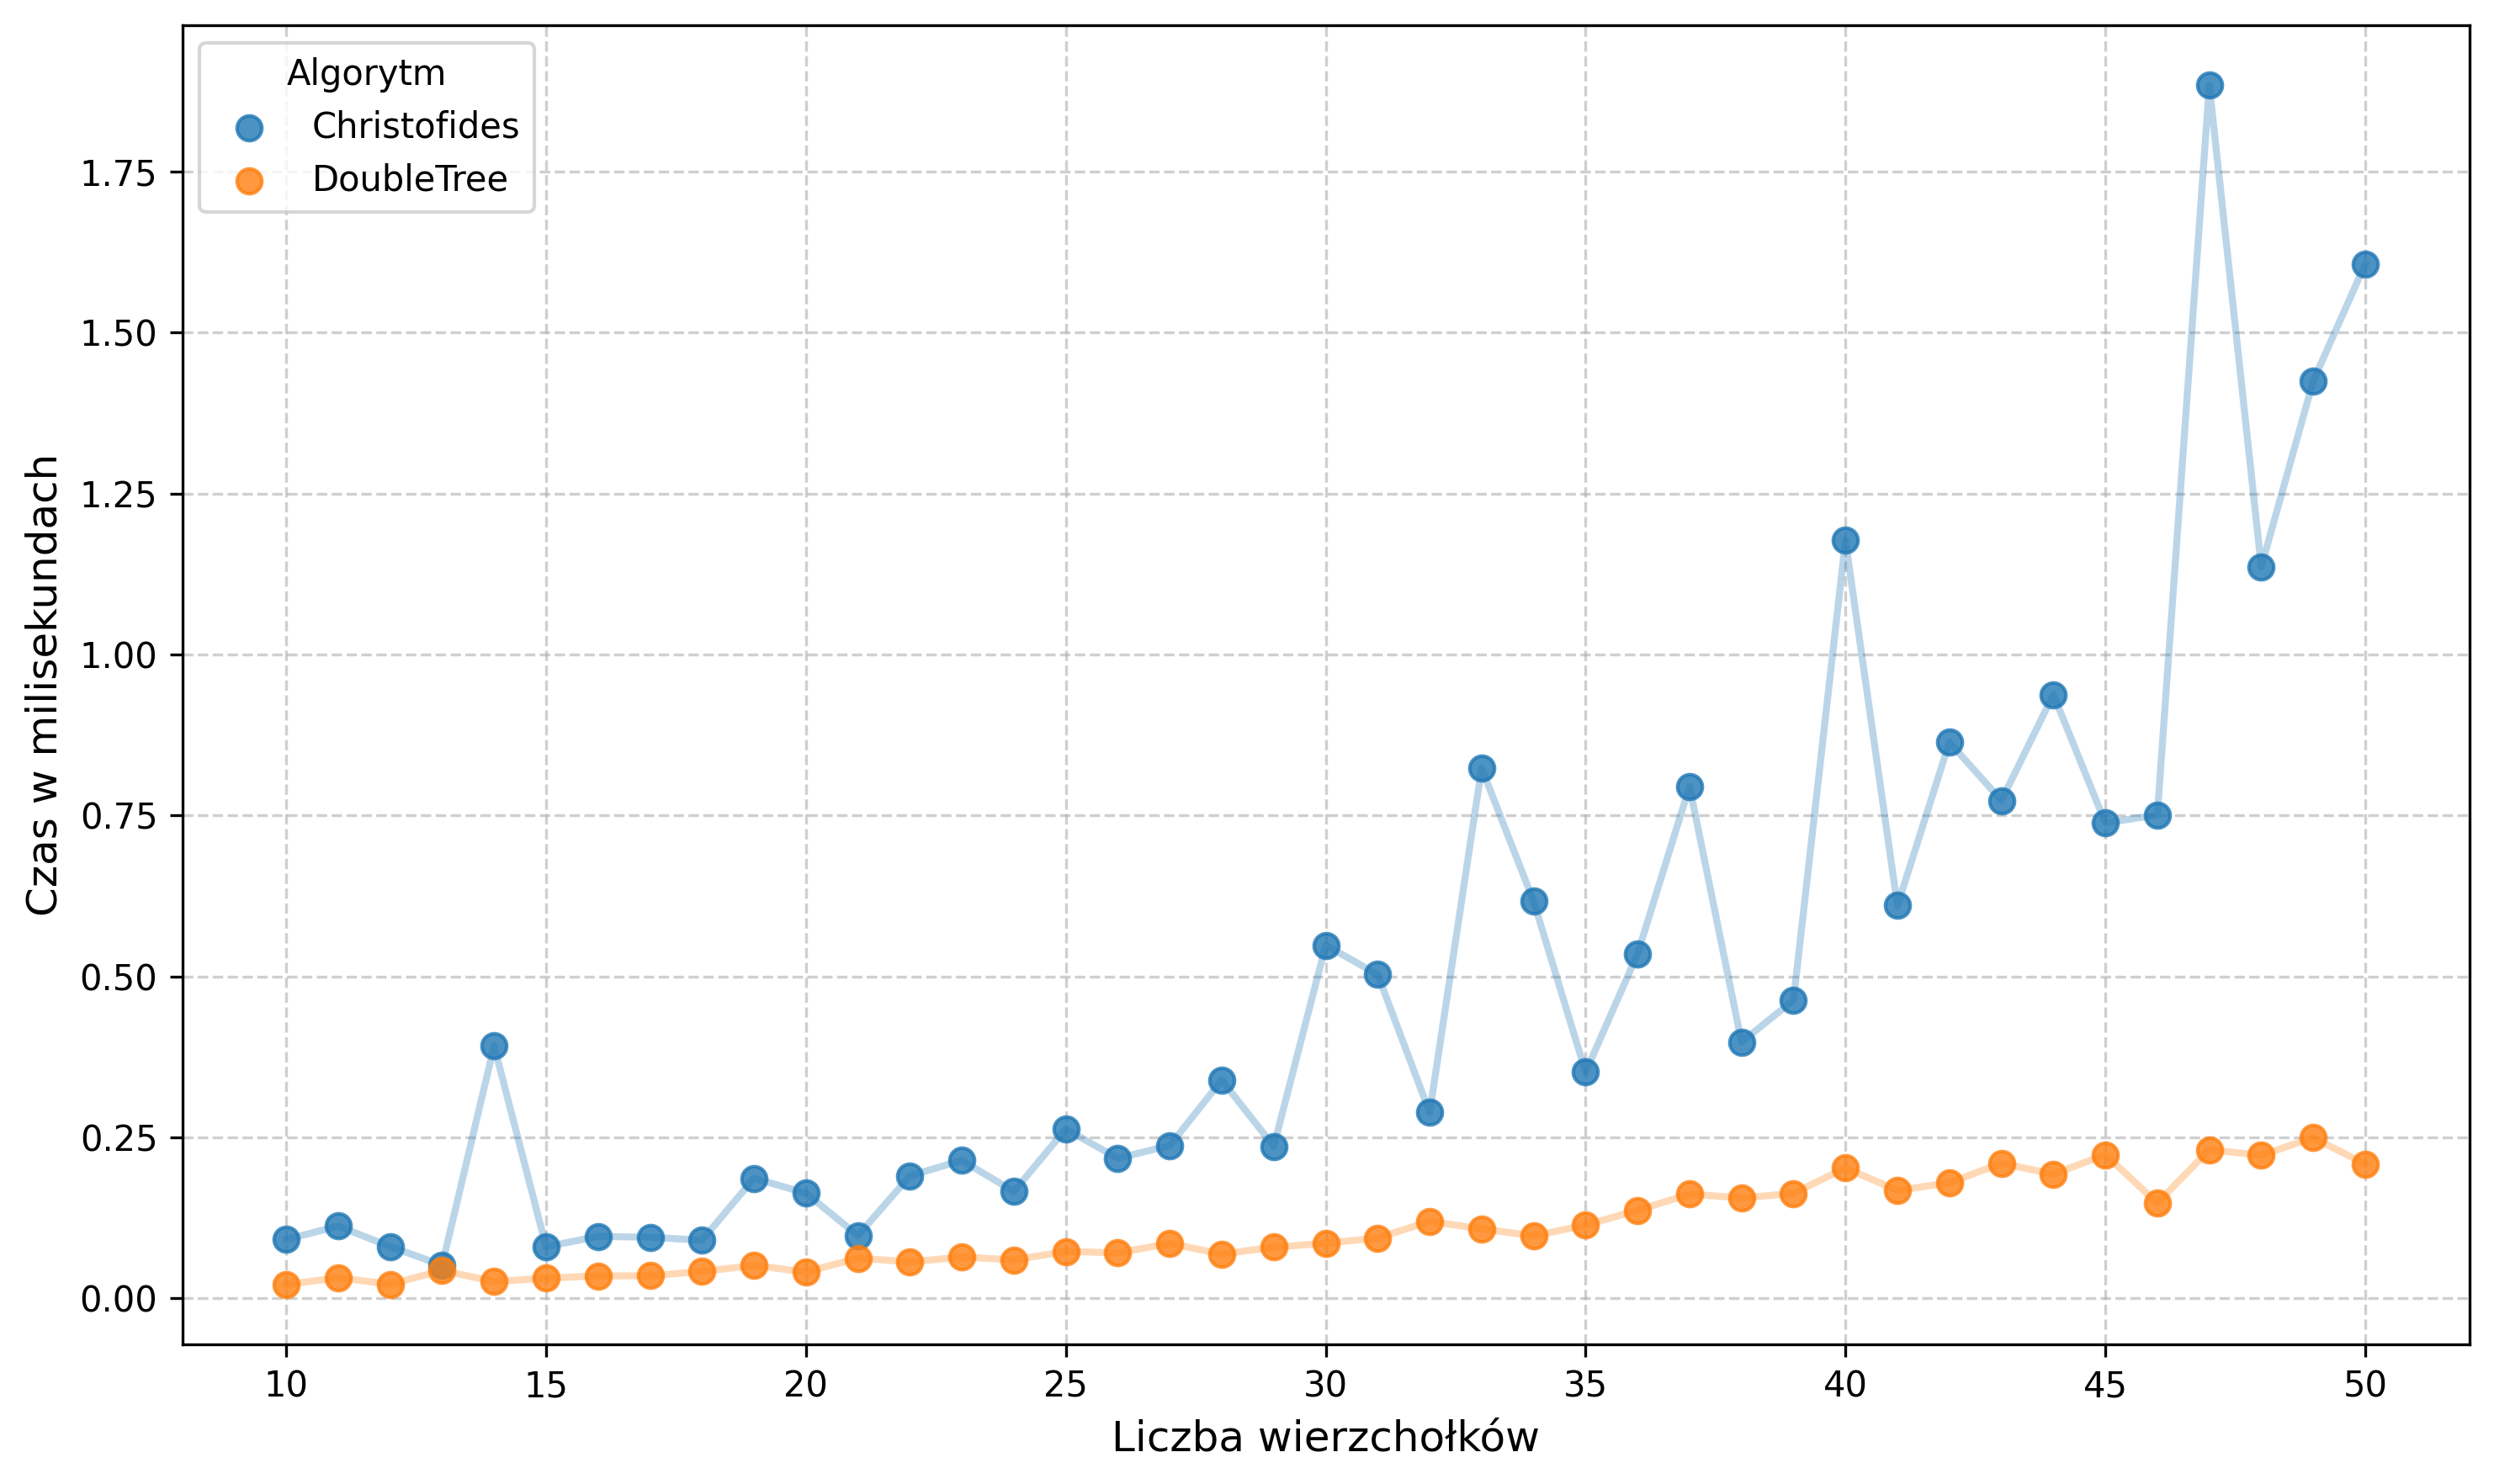
\includegraphics[width=0.9\textwidth]{images/random/small/small_time_complexity_plot.png}
    \caption{Porównanie czasu wykonania algorytmów Christofidesa i 2-aproksymacyjnego w funkcji liczby wierzchołków dla małych instancji losowych ($n \in [10, 50]$).}
    \label{fig:small_time_complexity}
\end{figure}

\subsubsection{Analiza dużych instancji losowych}
\label{subsubsec:czas_duze_instancje}

Przejście do analizy grafów o znacznie większej liczbie wierzchołków pozwala zaobserwować asymptotyczne różnice w złożoności obliczeniowej obu zaimplementowanych metod. Zestawienie wyników dla instancji w przedziale od $n=100$ do $n=500$ wierzchołków zaprezentowano na Rysunku \ref{fig:large_time_complexity}.

Algorytm 2-aproksymacyjny charakteryzuje się bardzo dobrą skalowalnością. Na wykresie zbiorczym krzywa reprezentująca ten algorytm przyjmuje postać niemal płaskiej linii, oscylującej tuż nad osią odciętych. Wyniki te potwierdzają, że oparcie aproksymacji wyłącznie na wyznaczaniu MST oraz przeszukiwaniu w głąb (DFS) gwarantuje wysoką wydajność nawet dla relatywnie dużych problemów.

Zupełnie inną dynamikę można zaobserwować w przypadku algorytmu Christofidesa, którego czas wykonania rośnie w sposób gwałtowny i nieliniowy. O ile dla grafów rzędu 100 wierzchołków algorytm ten potrzebuje około 20 ms, o tyle dla instancji największych ($n=490, n=500$) czas ten zbliża się do poziomu 350-380 ms. Krzywa odzwierciedla wielomianowy charakter wzrostu złożoności czasowej.

Podobnie jak w przypadku mniejszych instancji, algorytm Christofidesa wykazuje się wysoką wariancją w czasie wykonania –- szczególnie zauważalną w przedziale $n \in [350, 500]$, gdzie występują gwałtowne wahania i lokalne ekstrema. 

Przedstawione wyniki pokazują, że teoretyczna poprawa współczynnika aproksymacji w algorytmie Christofidesa wiąże się ze znaczącym i szybko rosnącym narzutem obliczeniowym.

\begin{figure}[H]
    \centering
    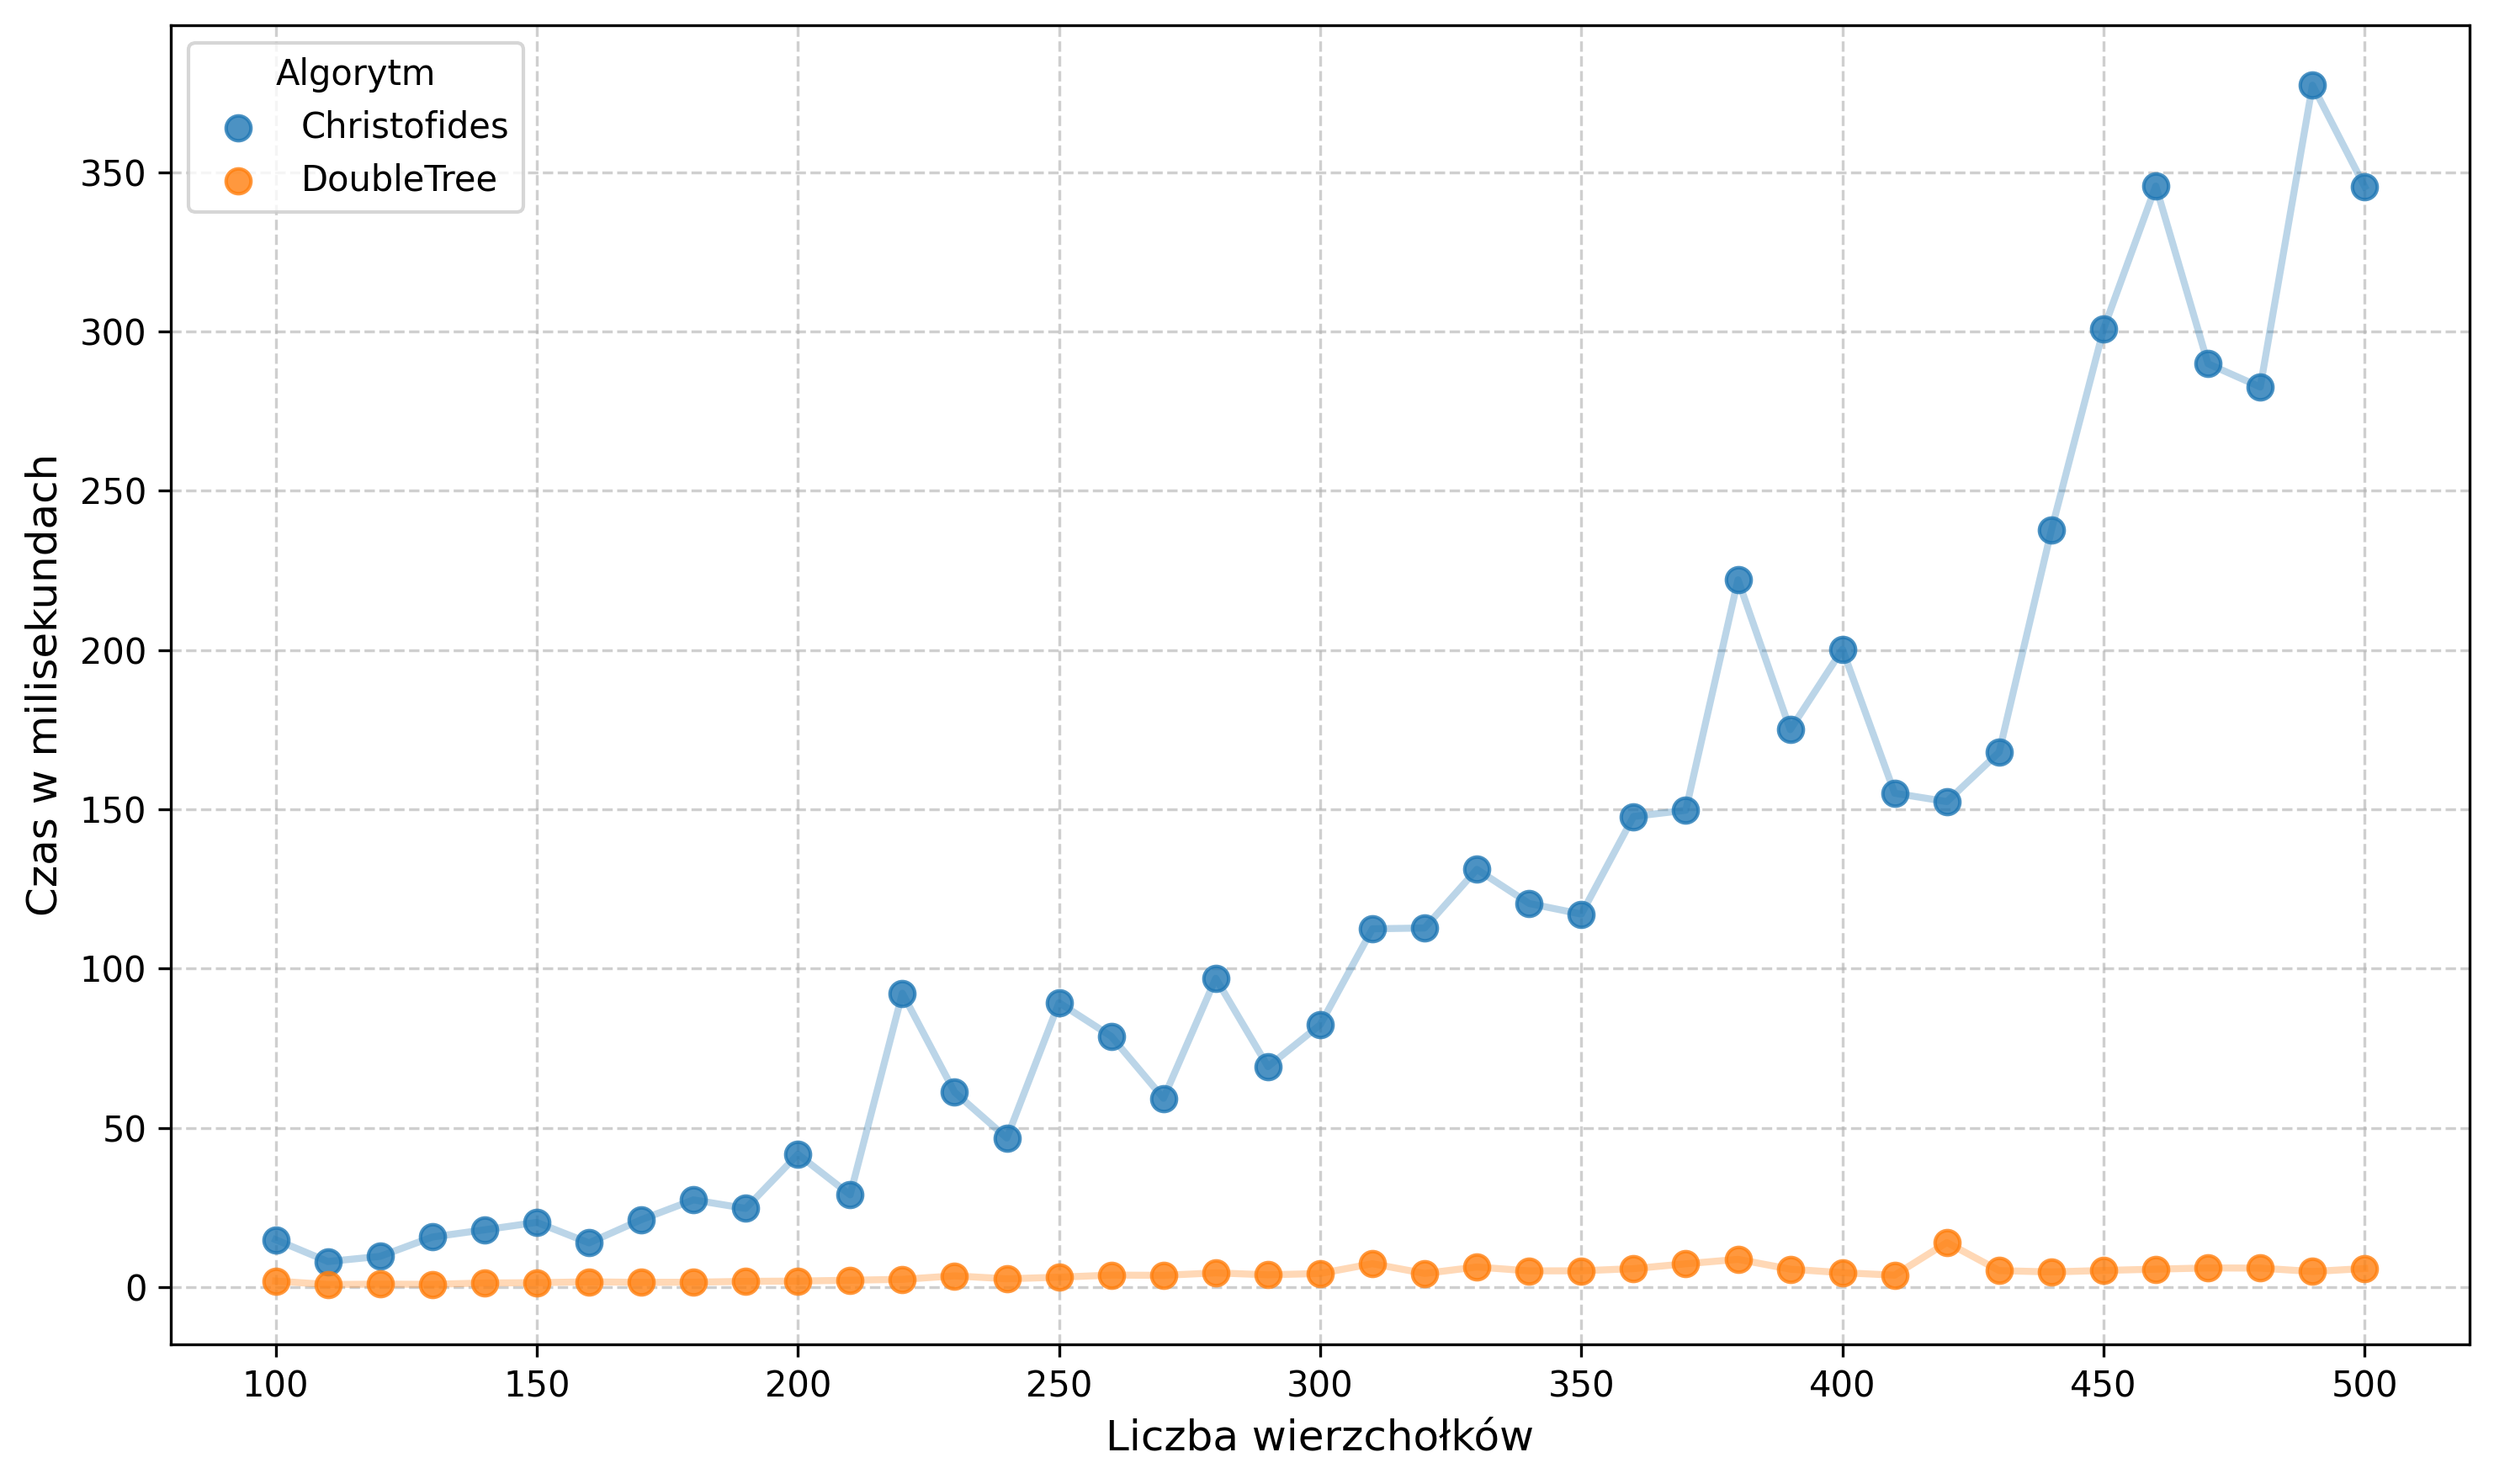
\includegraphics[width=0.9\textwidth]{images/random/large/large_time_complexity_plot.png}
    \caption{Porównanie czasu wykonania algorytmów Christofidesa i 2-aproksymacyjnego w funkcji liczby wierzchołków dla dużych instancji losowych ($n \in [100, 500]$).}
    \label{fig:large_time_complexity}
\end{figure}

\subsection{Jakość aproksymacji}
\label{subsec:jakosc_aproksymacji}

Do oceny jakości rozwiązań zwracanych przez zaimplementowane algorytmy wykorzystano referencyjny zbiór danych TSPLIB (\path{examples/tsplib/}), dla którego znane są globalne optima. Pozwoliło to na precyzyjne wyznaczenie \textbf{współczynnika aproksymacji}, definiowanego jako stosunek długości trasy wygenerowanej przez algorytm do długości trasy optymalnej. Wyniki eksperymentu, w funkcji rosnącej liczby wierzchołków $n$, zaprezentowano na Rysunku \ref{fig:approx_ratio}.

Dla ułatwienia analizy, na wykresie naniesiono poziome, przerywane linie w kolorze czerwonym, które reprezentują teoretyczne ograniczenia (górne granice błędu) dla obu analizowanych metod: 

\begin{itemize}
    \item współczynnik $1{,}5$ dla algorytmu Christofidesa oraz
    \item $2{,}0$ dla algorytmu 2-aproksymacyjnego.
\end{itemize}

\noindent
Analiza wykresu pozwala na sformułowanie kilku istotnych wniosków:

\begin{enumerate}
    \item \textbf{Wysoka skuteczność:} Jak wynika z wykresu, algorytm Christofidesa w praktyce radzi sobie zdecydowanie lepiej, niż wskazywałoby na to jego teoretyczne, pesymistyczne ograniczenie ($1{,}5$). Dla badanych instancji TSPLIB, empiryczny współczynnik aproksymacji oscyluje w wąskim paśmie, przyjmując wartości w przybliżeniu od $1{,}05$ do $1{,}15$. Oznacza to, że generowane trasy są zazwyczaj zaledwie o 5--15\% dłuższe od znanych optymalnych rozwiązań. Co więcej, wariancja jakości rozwiązań tego algorytmu jest relatywnie niska i nie wykazuje znaczącej tendencji wzrostowej wraz ze zwiększaniem rozmiaru instancji.
    
    \item \textbf{Wyższa wariancja i niższa jakość:} Zgodnie z przewidywaniami teoretycznymi, algorytm 2-aproksymacyjny generuje rozwiązania o zauważalnie niższej jakości. Otrzymane współczynniki charakteryzują się większym rozrzutem i mieszczą się przeważnie w przedziale $1{,}2 - 1{,}5$, przy czym dla pojedynczych instancji wartości te nieznacznie przekraczają próg $1{,}5$. Choć wszystkie wyniki pozostają z dużym marginesem poniżej teoretycznej granicy $2{,}0$, to wygenerowane ścieżki są średnio o 20--50\% gorsze od znanych optymalnych rozwiązań. Algorytm ten wykazuje również większą wrażliwość na topologię konkretnych instancji grafowych, co objawia się widocznymi fluktuacjami.
\end{enumerate}

\noindent
Algorytm 2-aproksymacyjny oferuje zwiększoną szybkość działania i skalowalność wraz z rozmiarem problemu (co udowodniono na dużych instancjach rzędu 500 wierzchołków), jednak odbywa się to kosztem zauważalnej utraty precyzji. Z kolei algorytm Christofidesa gwarantuje znalezienie trasy o wysokiej jakości, bliskiej optimum globalnemu, lecz wymaga zaakceptowania znaczącego wzrostu czasu obliczeń, co w przypadku bardzo dużych instancji może stanowić czynnik dyskwalifikujący.

\begin{figure}[H]
    \centering
    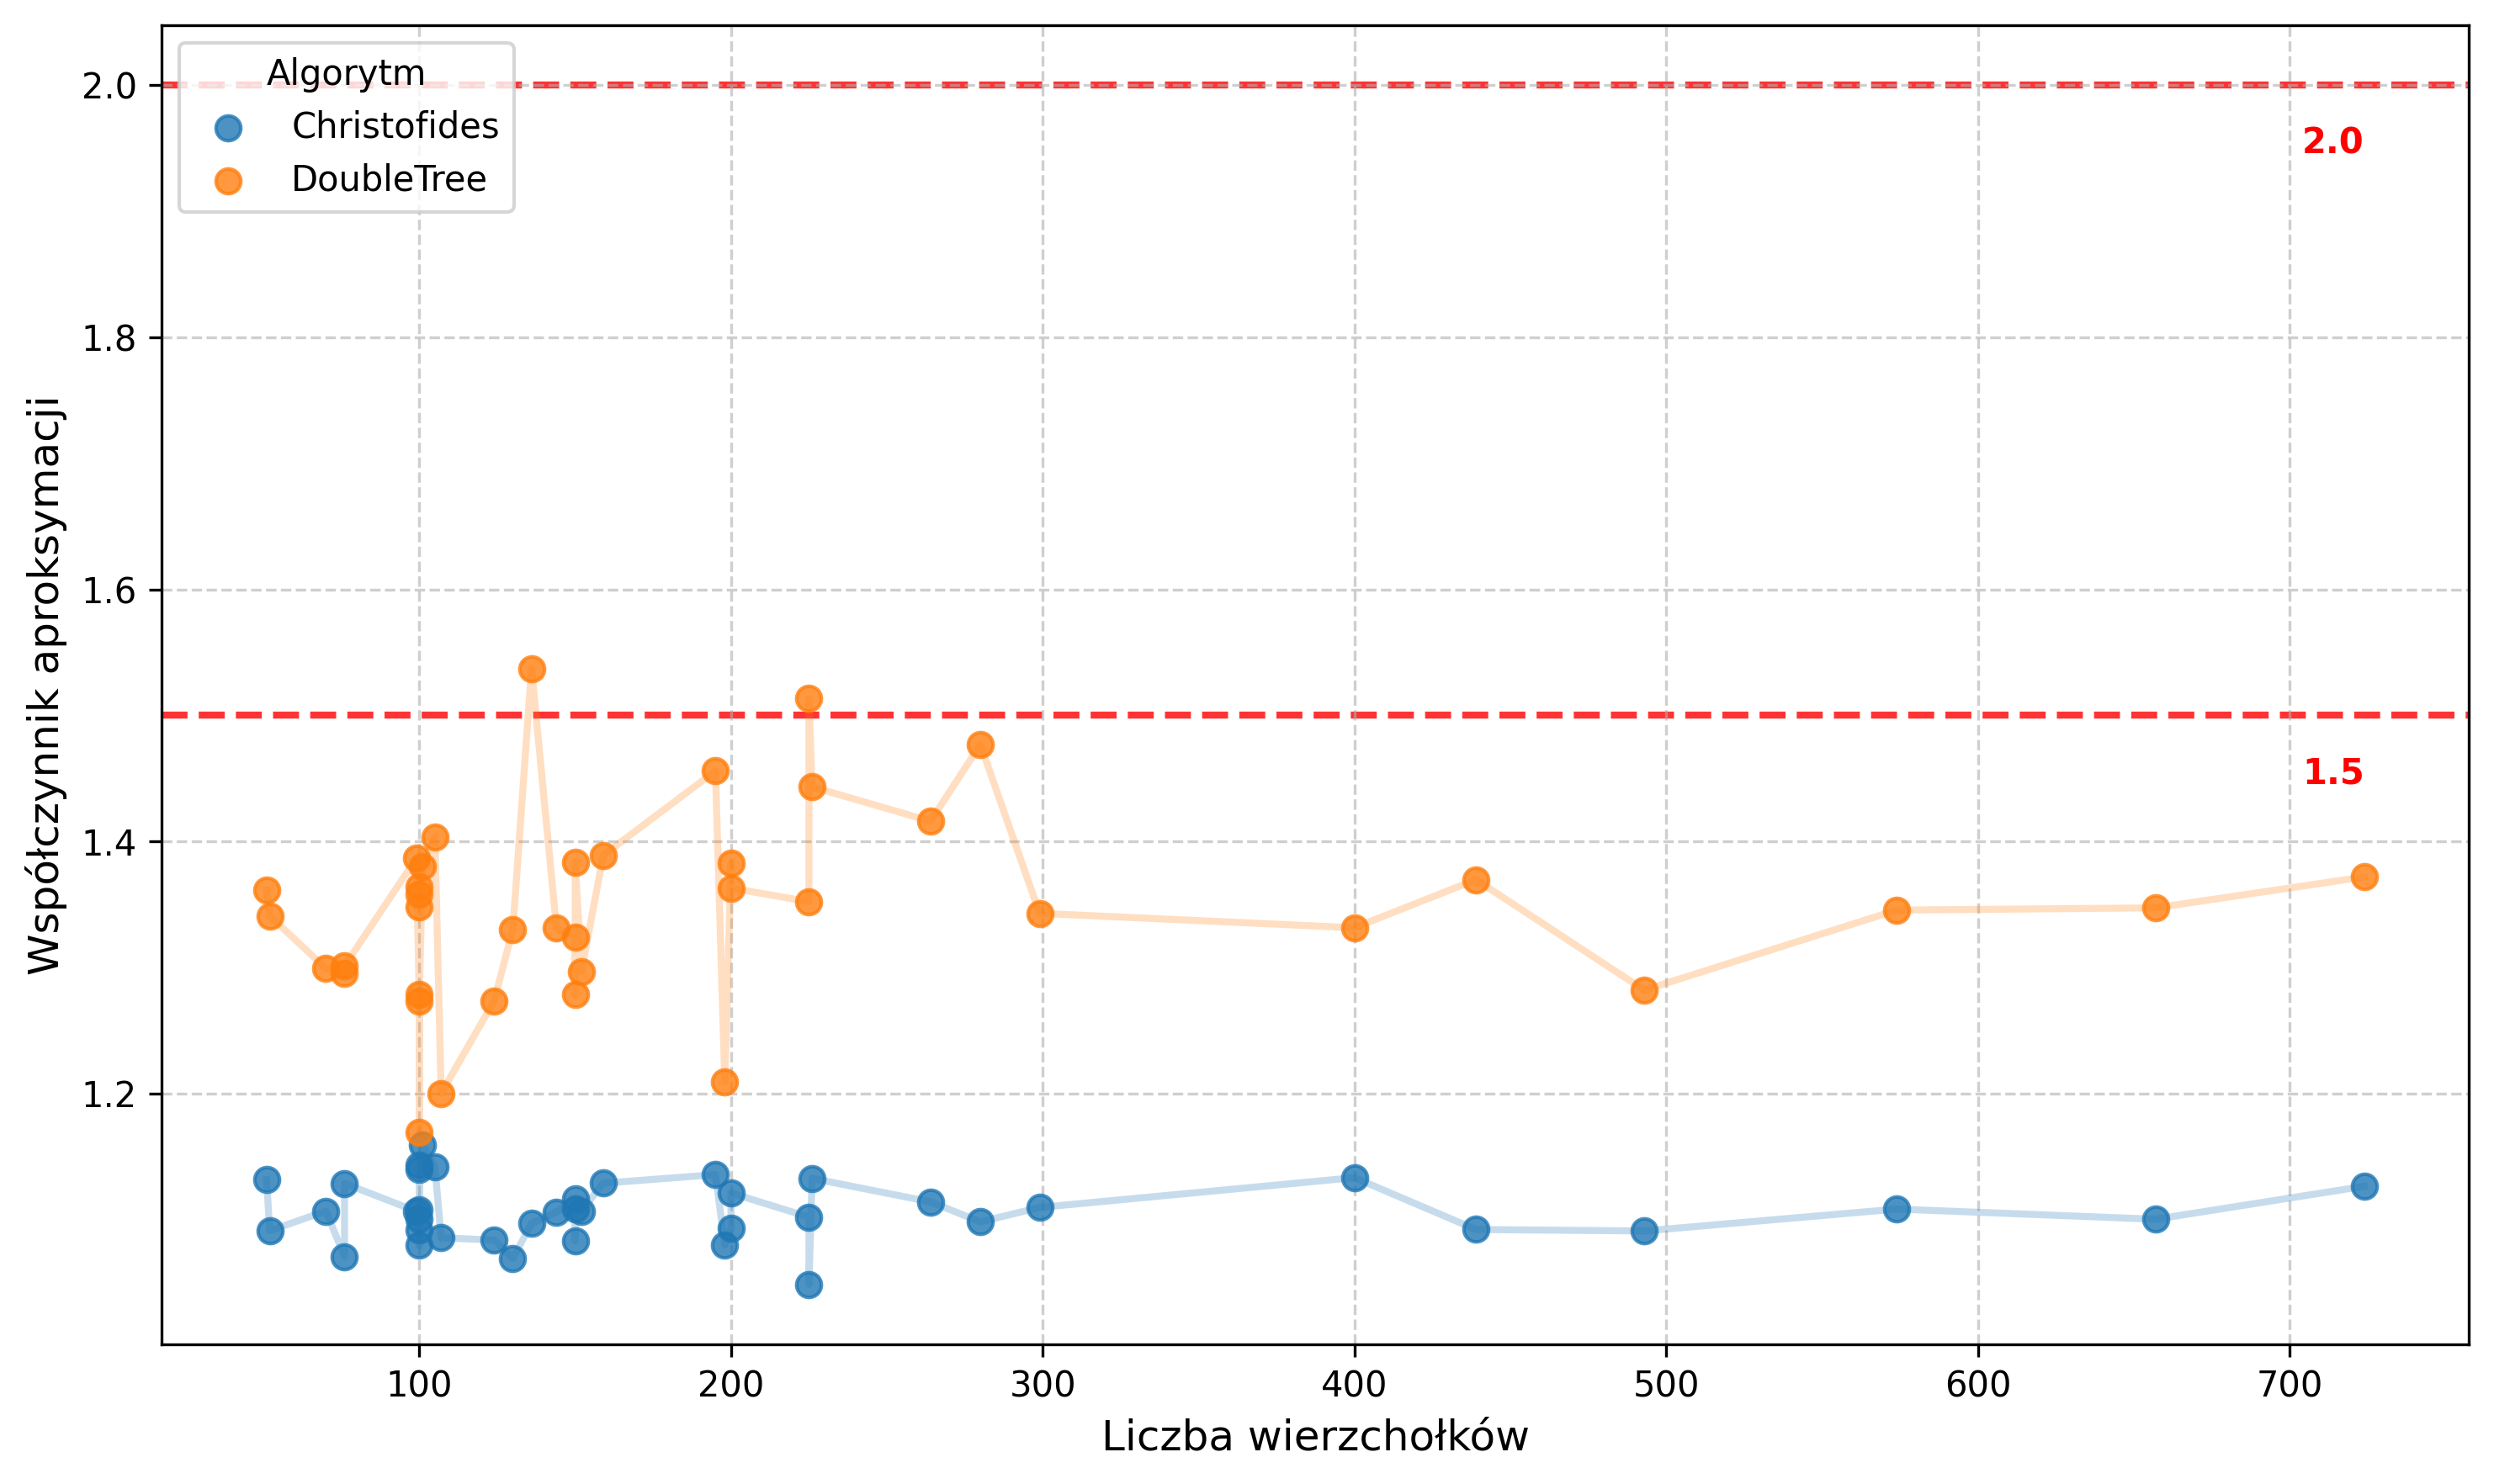
\includegraphics[width=1.0\textwidth]{images/tsplib/approximation_ratio_plot.png}
    \caption{Empiryczny współczynnik aproksymacji w funkcji liczby wierzchołków dla instancji z biblioteki TSPLIB. Czerwonymi przerywanymi liniami zaznaczono teoretyczne ograniczenia algorytmów ($1{,}5$ oraz $2{,}0$).}
    \label{fig:approx_ratio}
\end{figure}

\subsection{Analiza statystyczna błędu względnego}
\label{subsec:analiza_statystyczna}

Przeprowadzono szczegółową analizę statystyczną procentowego błędu względnego (odchylenia od optimum globalnego) dla referencyjnego zbioru 40 instancji TSPLIB. 

Podstawowe statystyki opisowe dla badanych metod zestawiono w Tabeli \ref{tab:statystyki_opisowe}, natomiast Rysunek \ref{fig:boxplot_error} prezentuje rozkład błędów w postaci wykresów pudełkowych.

\begin{table}[H]
    \centering
    \caption{Statystyki opisowe procentowego błędu względnego dla algorytmów Christofidesa i 2-aproksymacyjnego (próba $N=40$).}
    \label{tab:statystyki_opisowe}
    \renewcommand{\arraystretch}{1.0}
    \begin{tabular}{|l|c|c|}
        \hline
        \textbf{Statystyka} & \textbf{Christofides} & \textbf{2-aproksymacyjny} \\
        \hline
        Średnia [\%] & $10{,}67$ & $34{,}76$ \\
        Mediana [\%] & $10{,}66$ & $34{,}76$ \\
        Minimum [\%] & $4{,}84$ & $16{,}90$ \\
        Maksimum [\%] & $15{,}90$ & $53{,}72$ \\
        Odchyl. stand. [\%] & $2{,}34$ & $7{,}62$ \\
        \hline
    \end{tabular}
\end{table}

\noindent
Mediana błędu dla algorytmu Christofidesa wynosi zaledwie $10{,}66\%$, podczas gdy dla algorytmu 2-aproksymacyjnego osiąga poziom $34{,}76\%$. Algorytm Christofidesa charakteryzuje się bardzo zwartym rozkładem wyników -- rozstęp międzykwartylowy jest wąski, odchylenie standardowe wynosi jedynie $2{,}34\%$, a maksymalny zaobserwowany błąd nie przekracza $16\%$. 

Z kolei algorytm 2-aproksymacyjny wykazuje ponad trzykrotnie większe odchylenie standardowe ($7{,}62\%$). Na wykresie pudełkowym można zaobserwować obecność wartości odstających (w tym pojedynczych instancji z błędem przekraczającym $50\%$), co świadczy o znacznej wrażliwości na specyficzną strukturę grafu. Najlepszy wynik dla 2-aproksymacyjnego (błąd $16{,}90\%$) wypada gorzej niż najgorszy wynik dla Christofidesa (błąd $15{,}90\%$).

\subsubsection{Weryfikacja hipotez statystycznych}

Aby wykazać istotność statystyczną zaobserwowanych dysproporcji w jakości rozwiązań, przeprowadzono wnioskowanie statystyczne. Ponieważ badane próby są zależne (oba algorytmy testowano na tych samych instancjach problemu), do porównania wykorzystano test Wilcoxona (ang. \textit{Wilcoxon Signed-Rank Test})~\cite{wilcoxon1945individual}. 

Weryfikacji poddano hipotezę zerową ($H_0$), zakładającą brak istotnej statystycznie różnicy między medianami błędów względnych obu algorytmów. Przyjęto standardowy poziom istotności $\alpha = 0{,}05$. Zastosowanie testu dla $40$ par wyników pozwoliło na wyznaczenie wartości statystyki testowej $W = 0{,}0$ oraz odpowiadającej jej wartości prawdopodobieństwa testowego (ang. \textit{p-value}) wynoszącej $p \approx 1{,}82 \cdot 10^{-12}$. 

Uzyskane $p\text{-value}$ jest znacząco mniejsze od założonego poziomu istotności ($p < \alpha$), zatem \textbf{hipoteza zerowa zostaje odrzucona}. Różnica w jakości rozwiązań generowanych przez oba algorytmy jest wysoce istotna statystycznie, z jednoznacznym wskazaniem na algorytm Christofidesa w kontekście precyzji aproksymacji.

\begin{figure}[htbp]
    \centering
    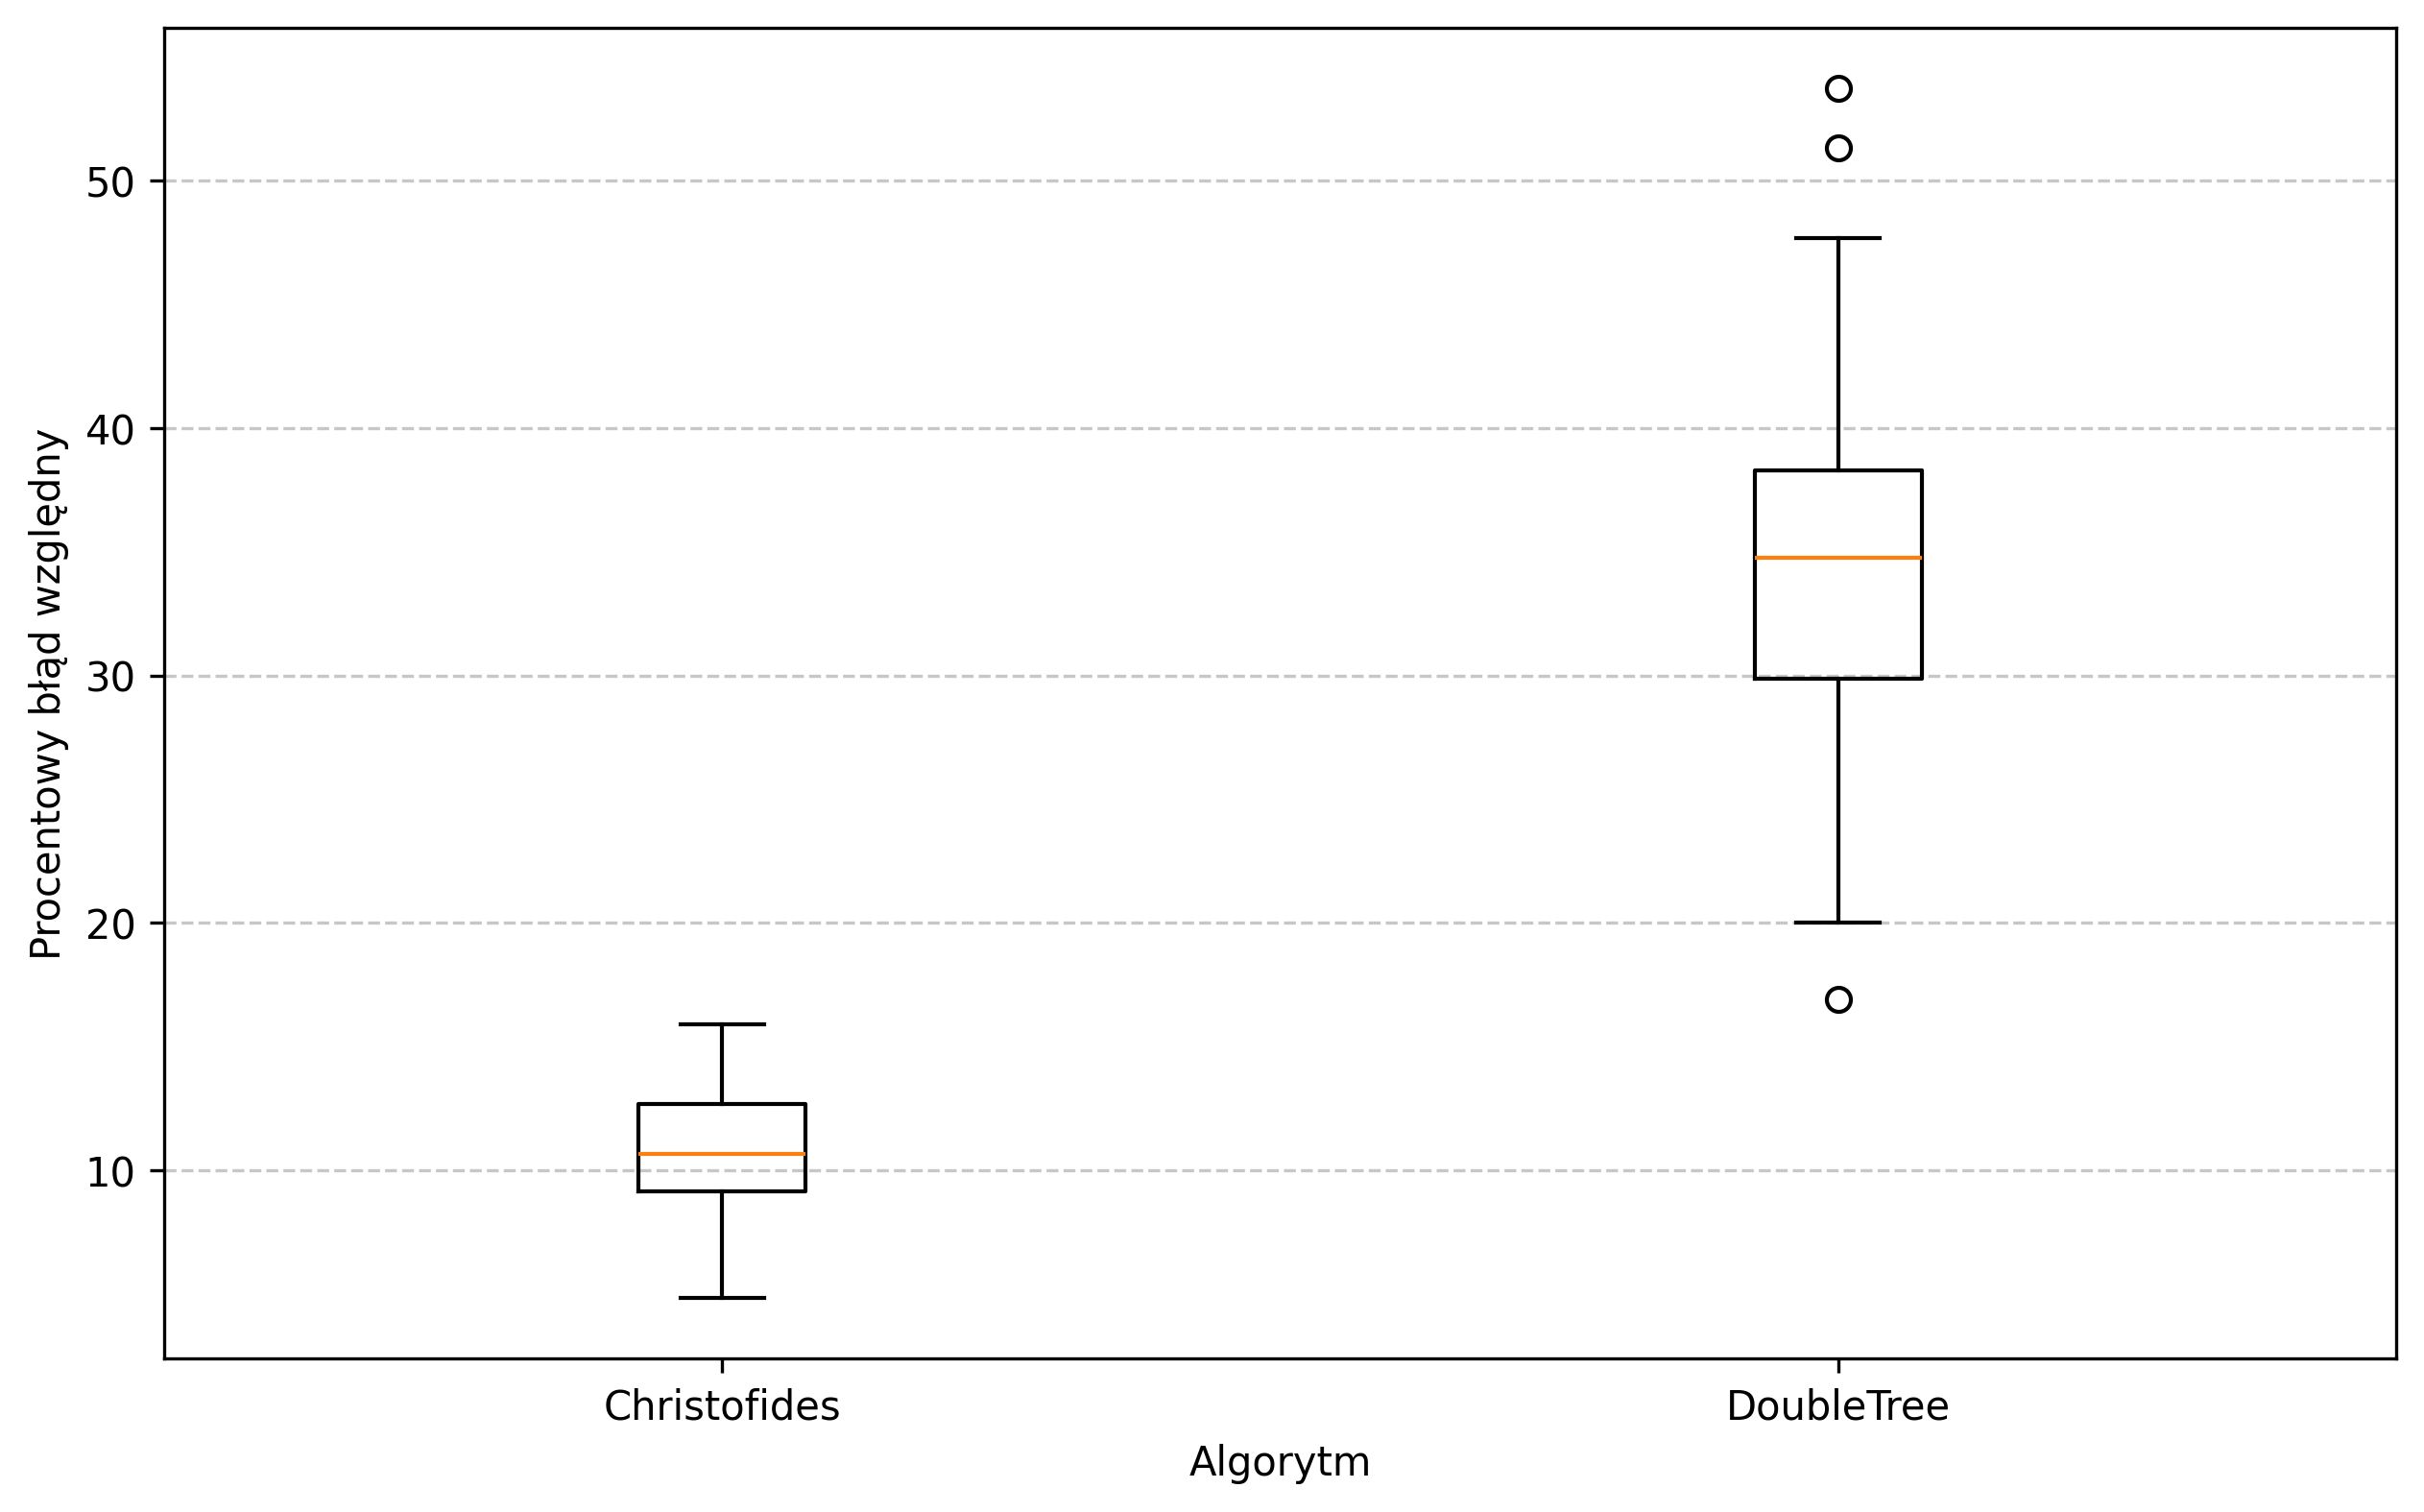
\includegraphics[width=0.9\textwidth]{images/tsplib/relative_error_boxplot.png}
    \caption{Rozkład procentowego błędu względnego dla badanych algorytmów (wykres pudełkowy). Centralna linia pudełka oznacza medianę, krawędzie wyznaczają kwartyle (Q1 i Q3), natomiast punkty reprezentują wartości odstające.}
    \label{fig:boxplot_error}
\end{figure}

\subsection{Zależność błędu aproksymacji od rozmiaru problemu}
\label{subsec:korelacja_bledu}

Z punktu widzenia praktycznych zastosowań algorytmów aproksymacyjnych istotne jest zweryfikowanie, czy jakość zwracanych rozwiązań ulega pogorszeniu wraz ze wzrostem rozmiaru instancji problemu. W tym celu dla instancji z biblioteki TSPLIB wyznaczono linie trendu oraz obliczono współczynniki korelacji między liczbą wierzchołków a procentowym błędem względnym. Wizualizację tej zależności przedstawiono na Rysunku \ref{fig:correlation_plot}.

Analiza metryk statystycznych, w tym współczynnika korelacji liniowej Pearsona ($r$)~\cite{pearson1895note} oraz korelacji rang Spearmana ($\rho$)~\cite{spearman1904proof}, ujawnia odmienną specyfikę badanych metod:
\begin{itemize}
    \item \textbf{Algorytm Christofidesa:} Wykazuje niemal całkowity brak korelacji pomiędzy rozmiarem grafu a wielkością popełnianego błędu ($r = 0{,}0040$, $\rho = 0{,}0123$). Linia trendu dla tego algorytmu jest praktycznie pozioma i stabilnie oscyluje wokół wartości 10--11\%. Algorytm potrafi utrzymać wysoką precyzję niezależnie od tego, czy przetwarza graf o kilkudziesięciu, czy kilkuset wierzchołkach.
    \item \textbf{Algorytm 2-aproksymacyjny:} Wykazuje słabą korelację dodatnią ($r = 0{,}1289$, $\rho = 0{,}2804$). Choć linia trendu zauważalnie wznosi się wraz ze wzrostem liczby wierzchołków, zależność ta nie jest na tyle silna, by dyskwalifikować algorytm dla dużych instancji. Potwierdza to jednak wcześniejsze obserwacje o wyższej wariancji i ogólnej mniejszej stabilności optymalizacyjnej algorytmu opartego wyłącznie na podwójnym drzewie rozpinającym.
\end{itemize}

\begin{figure}[H]
    \centering
    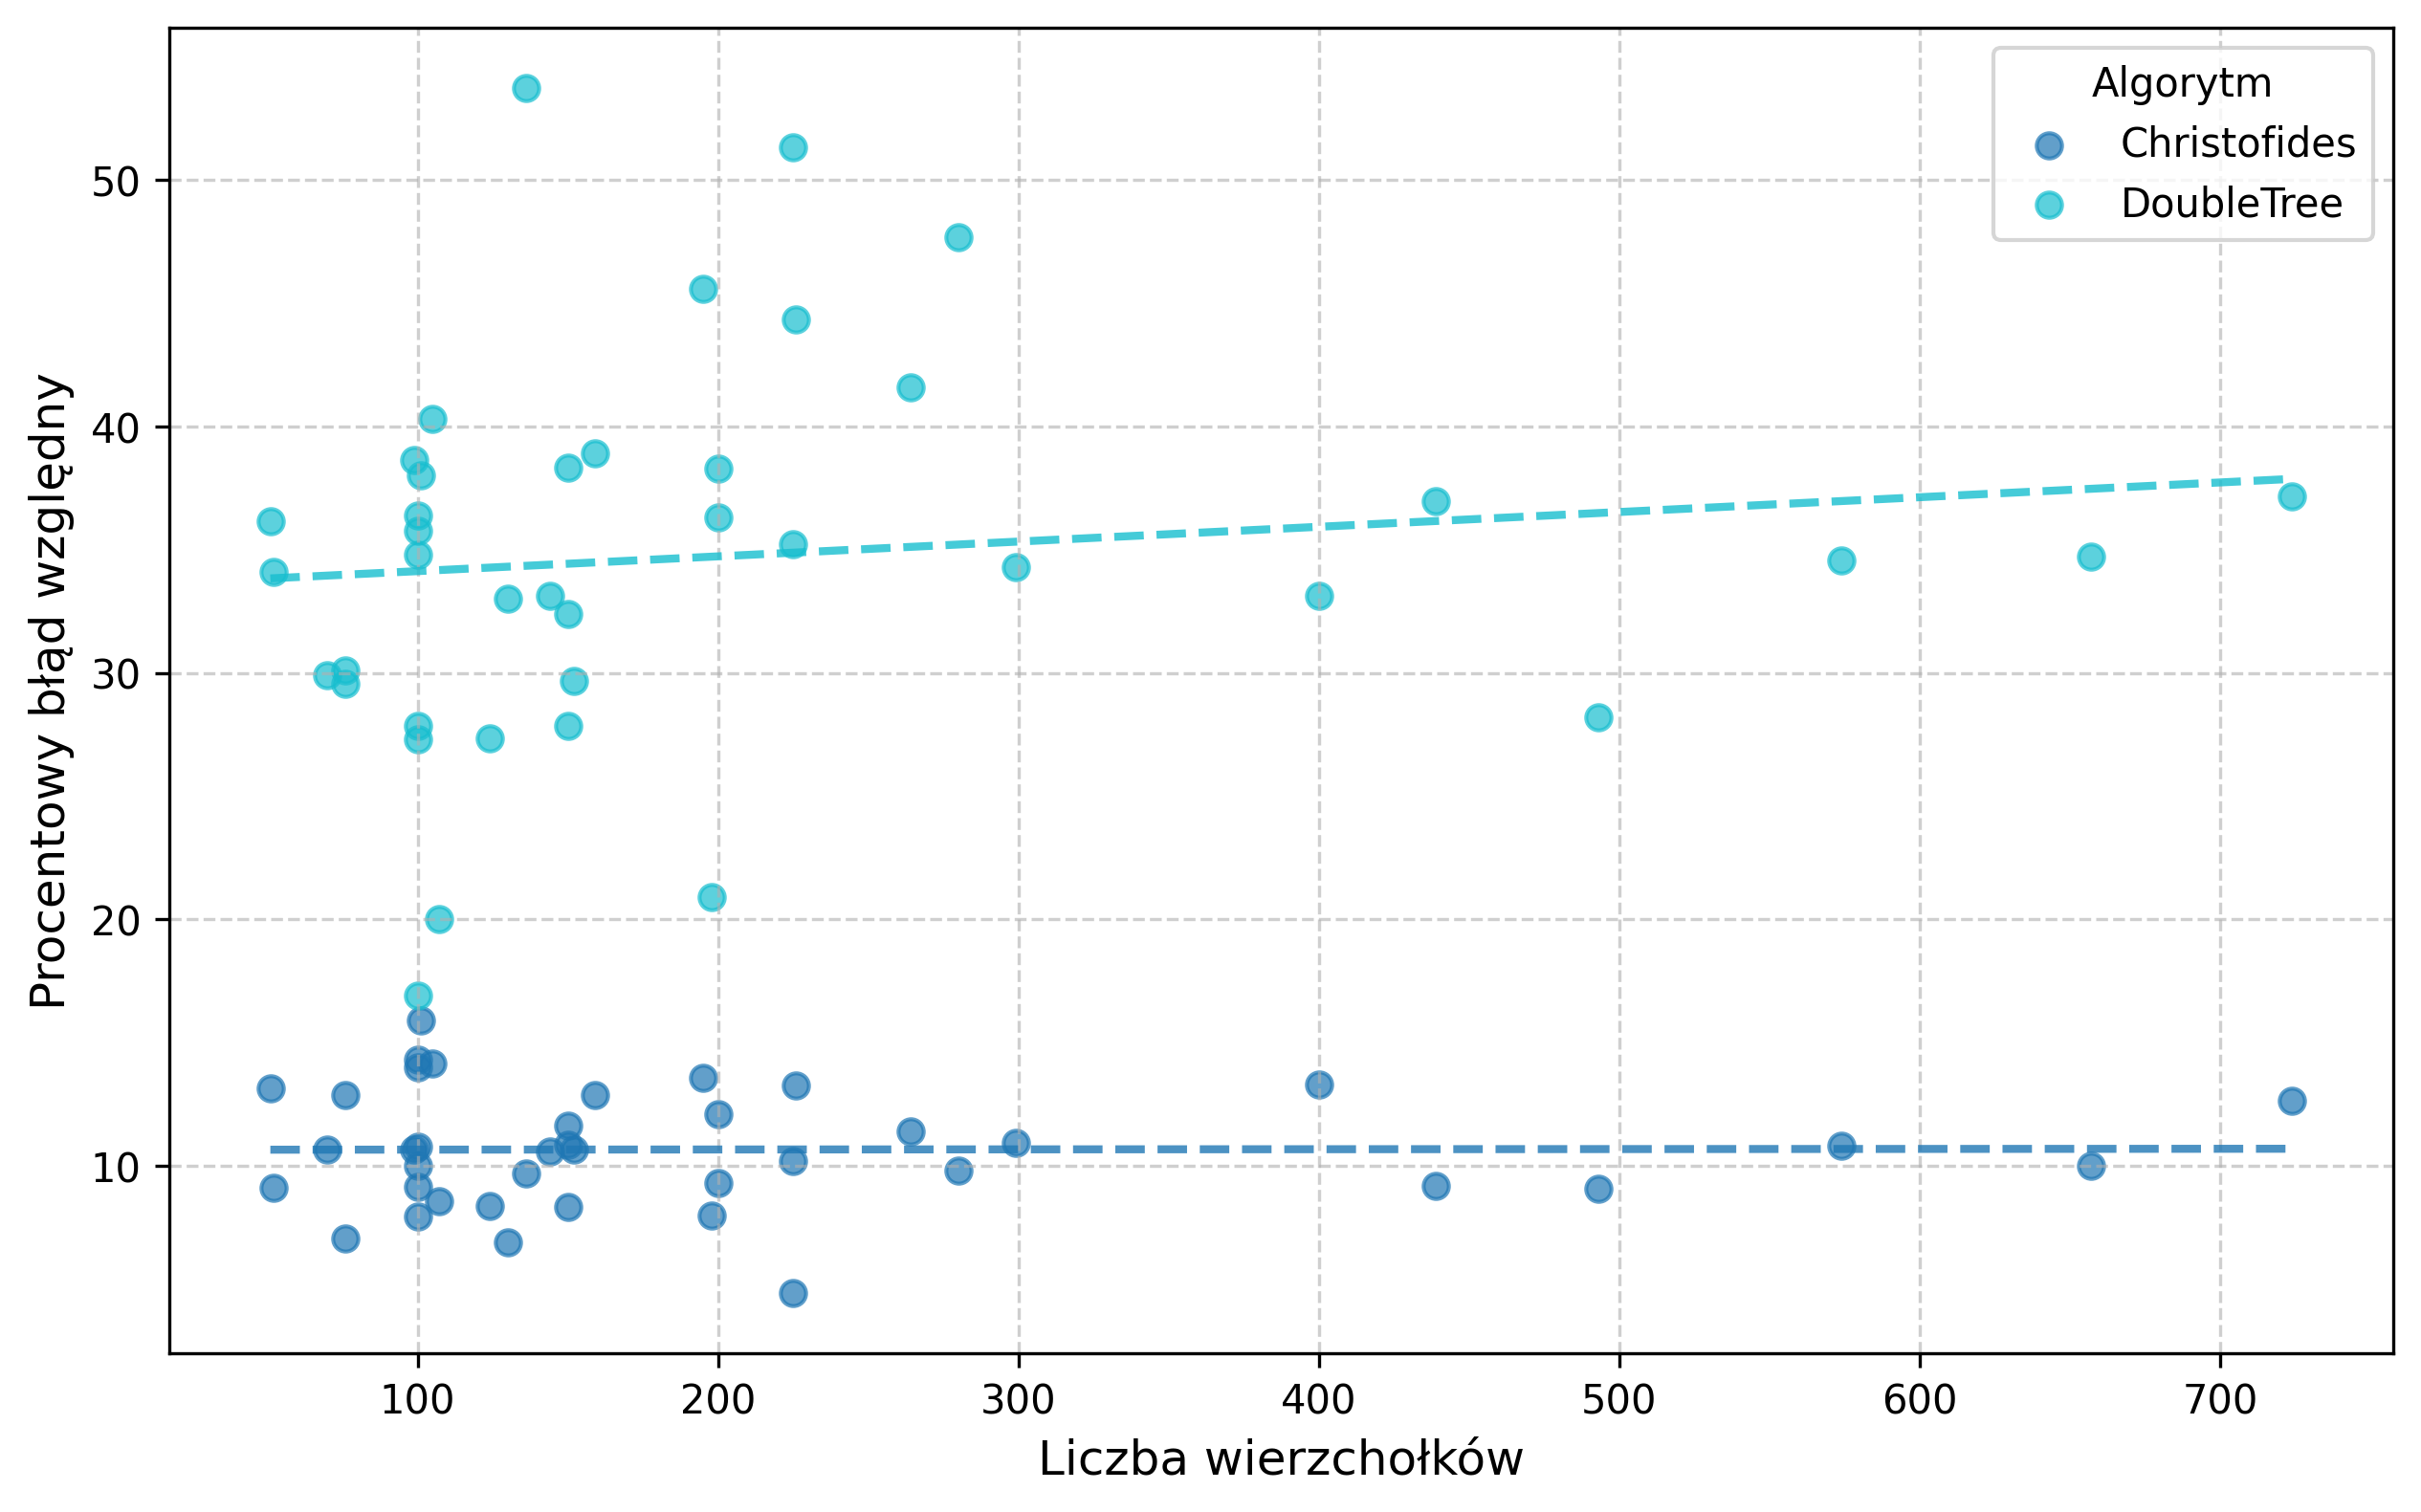
\includegraphics[width=0.9\textwidth]{images/tsplib/correlation_plot.png}
    \caption{Wykres rozrzutu ilustrujący zależność procentowego błędu względnego od liczby wierzchołków wraz z wyznaczonymi liniami trendu.}
    \label{fig:correlation_plot}
\end{figure}

\subsection{Czas obliczeń a precyzja}
\label{subsec:tradeoff}

Ostatecznym podsumowaniem przeprowadzonych eksperymentów jest bezpośrednie zestawienie dwóch rywalizujących ze sobą wskaźników wydajnościowych: czasu wykonania oraz wielkości procentowego błędu względnego. Rysunek \ref{fig:tradeoff_plot} prezentuje to zestawienie w postaci wykresu rozrzutu. Ze względu na różnice w narzucie obliczeniowym obu algorytmów (różnice rzędu kilku wielkości), oś odciętych (czas w milisekundach) została przedstawiona w skali logarytmicznej. \\

\noindent
W przestrzeni wyników formują się dwie, wyraźnie odseparowane od siebie chmury punktów:
\begin{enumerate}
    \item \textbf{Szybkość kosztem jakości:} Punkty reprezentujące algorytm 2-aproksymacyjny są wyraźnie przesunięte do lewej krawędzi wykresu (bardzo niskie czasy wykonania, od ułamków do kilkunastu milisekund), wykazując jednocześnie duży rozrzut wzdłuż osi rzędnych (błędy w przedziale 20--55\%). Jest to algorytm dedykowany dla systemów, w których szybkość podjęcia decyzji jest priorytetem, a gorsza jakość wyznaczonej trasy jest kosztem w pełni akceptowalnym.
    \item \textbf{Jakość kosztem czasu:} Reprezentacja wyników dla algorytmu Christofidesa tworzy wąskie, spłaszczone pasmo w dolnej sekcji wykresu (błędy utrzymane konsekwentnie poniżej 16\%), które jednak rozciąga się w prawo na osi logarytmicznej (osiągając czasy rzędu $10^3$ ms). Implementacja ta jest zatem uzasadniona w zastosowaniach, w których koszt samego procesu obliczeniowego jest pomijalny w stosunku do realnych oszczędności wynikających z odnalezienia trasy bliskiej optimum.
\end{enumerate}

\begin{figure}[H]
    \centering
    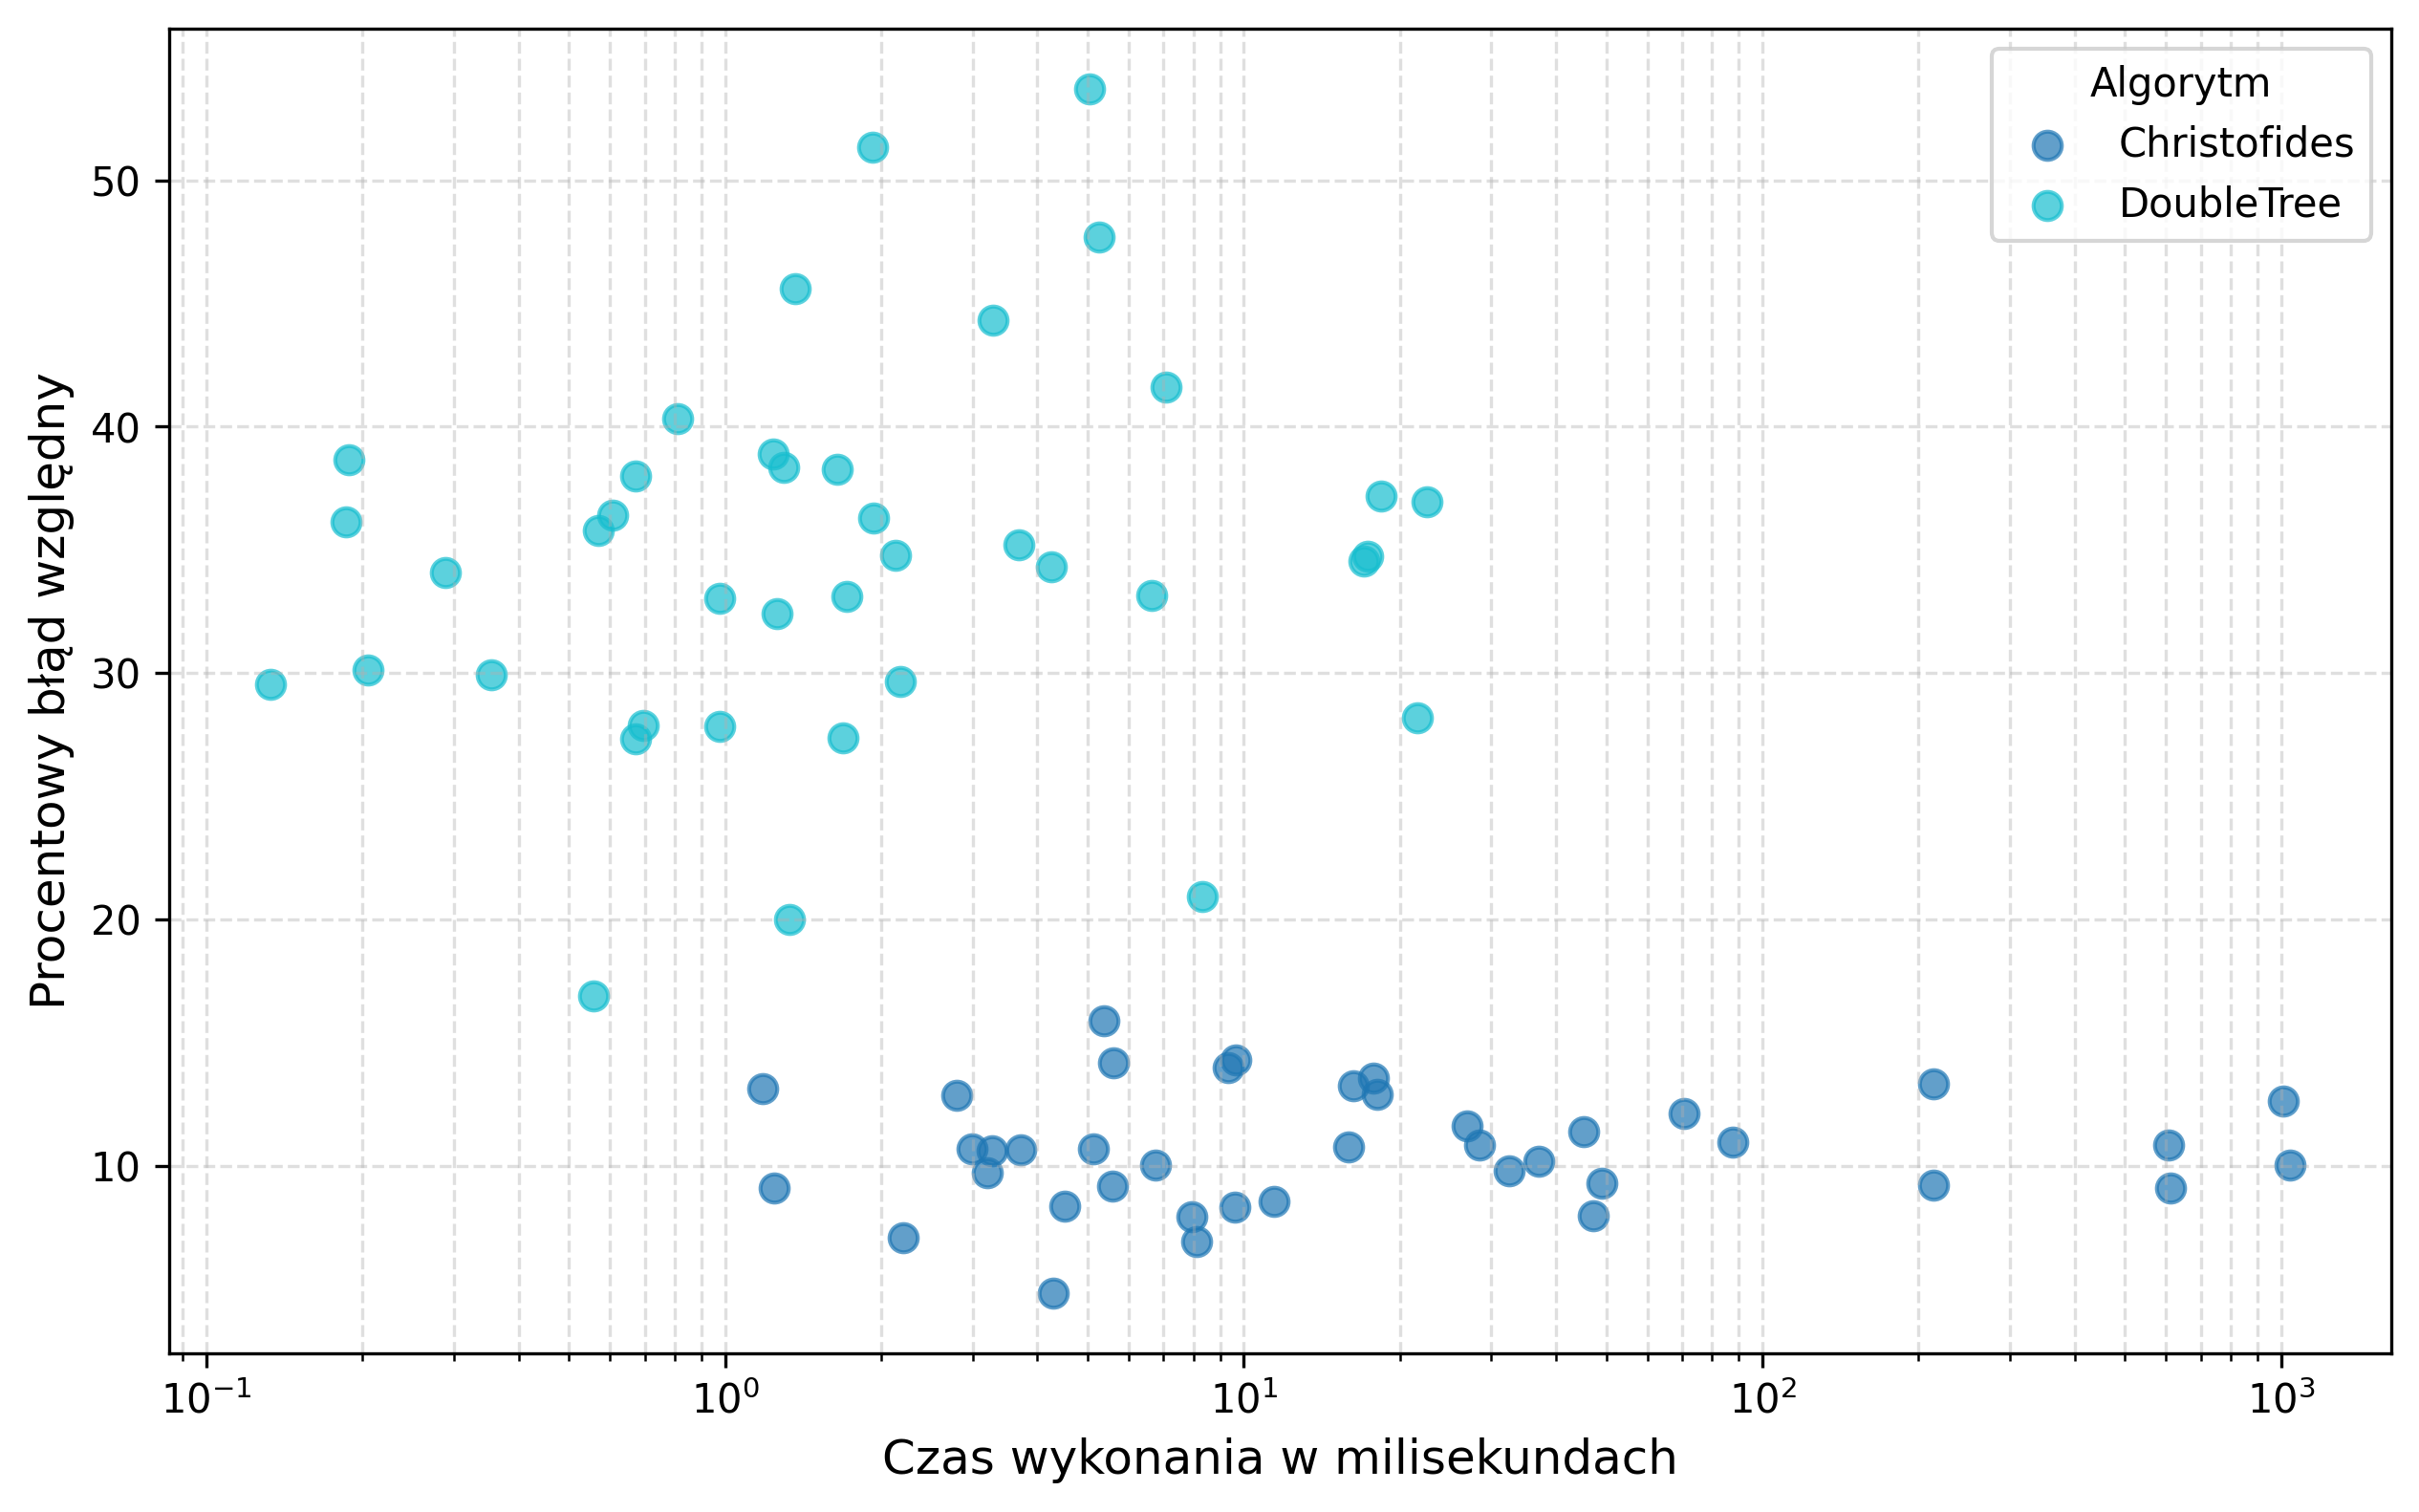
\includegraphics[width=0.9\textwidth]{images/tsplib/tradeoff_plot.png}
    \caption{Zestawienie kompromisu pomiędzy czasem wykonania (skala logarytmiczna) a procentowym błędem względnym dla referencyjnych instancji z biblioteki TSPLIB.}
    \label{fig:tradeoff_plot}
\end{figure}

\newpage
\section{Podsumowanie}
\label{sec:podsumowanie}

W ramach projektu zaimplementowaliśmy i porównaliśmy dwa algorytmy aproksymacyjne rozwiązujące metryczny problem komiwojażera (TSP): algorytm 2-aproksymacyjny (wykorzystujący podwójne drzewo rozpinające) oraz algorytm Christofidesa. Ponadto napisaliśmy własny generator instancji testowych oraz stworzyliśmy narzędzia do automatyzacji badań i wizualizacji wyników.

Aby ocenić skuteczność obu metod, przeprowadziliśmy serię eksperymentów na trzech zestawach danych: małych i dużych grafach wygenerowanych losowo (od 10 do 500 wierzchołków) oraz na referencyjnych instancjach z biblioteki TSPLIB. Zbadaliśmy przede wszystkim dwa aspekty: czas działania algorytmów oraz jakość wyznaczanych tras (czyli to, jak bardzo znaleziona ścieżka różni się od tej optymalnej).

Nasze badania pokazały wyraźny kompromis między szybkością a precyzją obliczeń. Najważniejsze wnioski płynące z eksperymentów są następujące:
\begin{itemize}
    \item \textbf{Algorytm 2-aproksymacyjny jest bardzo szybki i świetnie się skaluje.} Rozwiązywanie problemów dla grafów o wielkości 500 wierzchołków zajmuje mu zaledwie kilka milisekund. Kosztem tej szybkości jest jednak niższa dokładność -- wyznaczone trasy są średnio o 35\% dłuższe od optymalnych, a same wyniki bywają niestabilne i mocno zależą od struktury grafu.
    \item \textbf{Algorytm Christofidesa daje dużo lepsze i stabilniejsze wyniki.} Znalezione przez niego rozwiązania są średnio zaledwie o 10--11\% dłuższe od optimum. Osiąga to jednak kosztem znacznie dłuższego czasu działania, który gwałtownie rośnie wraz z wielkością problemu (głównie ze względu na konieczność wyznaczania skojarzenia doskonałego).
\end{itemize}

\noindent
Testy statystyczne potwierdziły, że różnica w jakości między tymi algorytmami nie jest przypadkowa. Wybór konkretnej metody zależy więc od potrzeb. Jeśli zależy nam na natychmiastowej odpowiedzi systemu, lepszym rozwiązaniem będzie algorytm 2-aproksymacyjny. Z kolei w sytuacjach, gdzie zależy nam na wyznaczeniu trasy jak najbliższej optimum i możemy poczekać na wynik, warto postawić na algorytm Christofidesa.

\newpage
\section{Podział pracy}

\begin{tblr}[
	caption = {Podział pracy w zespole.},
	label   = {tab:podzial-pracy},
	]{
		colspec = {|X[1,l]|X[4,l]|},
		rowhead = 1,
		hlines,
		row{1}  = {font=\bfseries},
	}
	Osoba & Zadania \\
	Marcin Cieszyński &
	\begin{minipage}[t]{\linewidth}
		\begin{itemize}[nosep, leftmargin=*, topsep=2pt]
			\item Analiza jakości aproksymacji i złożoności obliczeniowej dla algorytmu 2-aproksymacyjnego.
			\item Implementacja algorytmu 2-aproksymacyjnego.
			\item Uruchomienie programu na instancjach testowych i zebranie wyników do plików CSV.
			\item Analiza wyników eksperymentów.
		\end{itemize}
	\end{minipage} \\
	Radosław Głasek &
	\begin{minipage}[t]{\linewidth}
		\begin{itemize}[nosep, leftmargin=*, topsep=2pt]
			\item Analiza jakości aproksymacji i złożoności obliczeniowej dla algorytmu Christofidesa.
			\item Analiza teoretyczna algorytmu Hierholzera oraz algorytmu Edmonds'a w wariancie pierwotno-dualnym.
			\item Implementacja algorytmu Christofidesa.
			\item Analiza wyników eksperymentów.
		\end{itemize}
	\end{minipage} \\
	Adam Grącikowski &
	\begin{minipage}[t]{\linewidth}
		\begin{itemize}[nosep, leftmargin=*, topsep=2pt]
			\item Specyfikacja oraz implementacja wejścia i wyjścia.
			\item Implementacja generatora instancji testowych.
			\item Wygenerowanie instancji losowych oraz przygotowanie instancji testowych z biblioteki TSPLIB do przeprowadzenia eksperymentów.
			\item Instrukcja użytkownika wraz z przykładami uruchomienia.
			\item Przygotowanie skryptów generujących wykresy dla wyników eksperymentów.
			\item Analiza wyników eksperymentów.
		\end{itemize}
	\end{minipage} \\
\end{tblr}

\newpage
\printbibliography
\end{document}